\documentclass[a4paper,12pt]{article}
\renewcommand{\baselinestretch}{1.5} 

\usepackage[utf8]{inputenc}
\usepackage[acronym,toc]{glossaries}
\usepackage{url}
\usepackage{booktabs}
\usepackage{appendix}
\usepackage{setspace} % for \onehalfspacing and \singlespacing macros
%\singlespacing
\usepackage{etoolbox}
\AtBeginEnvironment{quote}{\singlespacing\small}

%Necessary packages
\usepackage[english]{babel}
\usepackage{amsmath, amsthm, amssymb}
\usepackage{a4wide}
\usepackage{verbatim}
\usepackage{import}
%\usepackage{xparse}
\usepackage{enumerate}
\usepackage{pdflscape}
\def\sym#1{\ifmmode^{#1}\else\(^{#1}\)\fi}

%graphical packages
\usepackage{csvsimple}
\usepackage{float}
\usepackage{algorithm2e}
\usepackage{sidecap}
\usepackage{wrapfig}
\usepackage[final]{graphicx}
\usepackage[space]{grffile}
\usepackage{caption}
\usepackage{subcaption}
\usepackage[section]{placeins}
\usepackage{tikz}
\usepackage{color}
\usepackage{eurosym}
\usepackage{rotating}
\usepackage{amstext} % for \text
\usepackage{natbib}
\usepackage{hyperref}
\hypersetup{final}
\hypersetup{
    colorlinks=true,
    linkcolor=cyan,
    filecolor=cyan,      
    urlcolor=cyan,
    citecolor=cyan
}

%Indentation
\setlength\parindent{20pt}
%Theorems, Definition, ordered by section
\theoremstyle{plain}
\newtheorem{theorem}{Theorem}[section]
\theoremstyle{definition}
\newtheorem{definition}[theorem]{Definition}
\theoremstyle{definition}
\newtheorem{lemma}[theorem]{Lemma}
\theoremstyle{definition}
\newtheorem{proposition}[theorem]{Proposition}
\theoremstyle{definition}
\newtheorem{corollary}[theorem]{Corollary}


%%%%% Title %%%%%
\title{Agricultural child labour in response to climate change\footnote{This thesis constitutes the final deliverable for the Masters degree in Public Policy and Human Development, with a specialization in Social Protection Policy, at UNU-MERIT and Maastricht University.}}
\author{Author: Mathias Weidinger (i6113552)\footnote{Student in the M.Sc. Public Policy and Human Development programme, cohort September 2018, Maastricht University and UNU-MERIT, \href{mailto:m.weidinger@maastrichtuniversit.nl}{\texttt{m.weidinger@maastrichtuniversity.nl}}.}\\ Supervisor: Prof. Dr. Pierre Mohnen\footnote{Professor of Microeconometrics at Maastricht University, Professorial Fellow at UNU-MERIT.}}
\date{\today %\\ First version: November 2020
}

\begin{document}

\maketitle

\begin{abstract}
Anthropogenic climate change severely impacts agriculture in developing countries and with it the millions of children actively involved in that sector. Economic theory can be used to characterise the effects that climate change might have on agricultural child labour. Merging two strands of theoretical literature, from Environmental Economics and Development Economics, this paper presents a simple household decision model of child labour supply under climate change. To take the model to the data, I combine a household panel from Nigeria with geo-coded weather records and estimate the dose-response functions for temperature and precipitation. Higher mean-temperatures are estimated to increase climate change, whereas the effects of extreme weather events are mixed and highly non-linear.

% ADD some detail about the outcomes once they are available...and feed them into three models: structural estimates via maximum likelihood are compared with those obtained from a commonly used non-parametric method (B-splines) and those of the recently proposed spatial first difference estimator. 
\end{abstract}
% J22=Time allocation and labour supply
% J43=Agricultural Labour Markets
% I32=Measurement and Analysis of Poverty
% Q54=Climate, Natural Disasters, Global Warming
% D11=Consumer Economics: Theory
% D12=Consumer Economics Empirical Analysis
% D13 Household Production and intrahousehold allocation

\textit{JEL}: D11, D12, D13, J22, J43, I32, Q54

\textit{Keywords}: child labour, climate change, agriculture, global warming

\clearpage

%chapters:

\section*{Declaration of Academic Integrity}
I, Mathias Weidinger, hereby declare with relation to my master's thesis
\textit{Agricultural child labour in response to climate change} that:

\begin{itemize}
    \item I am aware of and have understood the rules and regulations stipulated in the Education and Examination Regulations (EER) regarding fraud and plagiarism;
    \item I am aware of the possible consequences and disciplinary measures in the case of fraud and plagiarism in my master's thesis;
    \item I have conducted myself in accordance with the Thesis Guidelines, Education and Examination Regulations and generally established standards of academic integrity in writing my master's thesis;
    \item I have carefully marked and referenced all direct quotes and references, and indirect quotes included in my master's thesis;
    \item my master's thesis is an original result of my own work and does not include the work of others except in the case of direct and indirect quotes that are recognizable as such.
\end{itemize}
\vspace{1cm}
\centering
Signed at Seewalchen am Attersee on \today.\\

\vspace{1cm}

\includegraphics{signature.png}

 \justifying
\clearpage

\section*{Dedication}
\vspace{1cm}
I would like to express my heartfelt gratitude to my peers, colleagues, and mentors. Without your input this thesis would not have seen the light of day.
\begin{itemize}
    \item [] To Professor Pierre Mohnen for his patience and guidance.
    \item [] To Patrick and Nina for sparking my interest in environmental economics, and to Oral for reminding me not to believe all stories economists might tell me.
    \item [] A los jóvenes de la Feria Líbre, a la Fundación PACES, a VoloB, y a mis hermanos de la comunidad Yanuncay - por plantar en mí el deseo de seguir su ejemplo de solidaridad vivida y humanidad sincera. Este labor no existiera si no fuera por la inspiración que me brindaron Ustedes.
    \item [] To my friends through space and time - life, like research, would be dull without you.
    \item [] To Nanaya, for believing in me beyond reason.
    \item [] To Mum and Dad for everything.
\end{itemize}

    \clearpage

\section*{List of abbreviations}

\textbf{2SLS} Two-stage Least Squares; 
\textbf{ARE} Agricultural, Resource and Environmental Economics; 
\textbf{CDD} Correlation Decay Distance; 
\textbf{CLD} Cloud Cover, CRU-TS; 
\textbf{CRE} Correlated Random Effects; 
\textbf{CRU-TS} Climatic Research Unit gridded Time Series; 
\textbf{DTR} Diurnal Temperature Range, CRU-TS; 
\textbf{EA} Enumeration Area, GHG; 
\textbf{EIA} Environmental Impact Assessment; 
\textbf{EKC} Environmental Kuznets Curve; 
\textbf{FAO} Food and Agricultural Organization of the United Nations; 
\textbf{FE} Fixed Effects; 
\textbf{FRS} Freezing Days, CRU-TS; 
\textbf{GCM} Global Climate Model; 
\textbf{GDP} Gross Domestic Product; 
\textbf{GHG} Green House Gas; 
\textbf{GHS} General Household Survey, Nigeria; 
\textbf{HIC} High Income Country; 
\textbf{HYV} High Yield Variety; 
\textbf{ILO} International Labour Organization; 
\textbf{IMF} International Monetary Fund; 
\textbf{IPCC} International Panel on Climate Change; 
\textbf{IPEC} International Programme on the Elimination of Child Labour, ILO; 
\textbf{LGA} Legislative Government Area, Nigeria; 
\textbf{LMIC} Low- and Middle Income Country; 
\textbf{LSMS} World Bank's Living Standards Measurement Surveys; 
\textbf{MPI} Multi-dimensional Poverty Index; 
\textbf{NAERLS} National Agricultural Extension and Research Liaison Services, Nigeria; 
\textbf{NBS} National Bureau of Statistics, Nigeria; 
\textbf{OLS} Ordinary Least Squares; 
\textbf{OPHI} Oxford Poverty and Human Development Initiative; 
\textbf{PET} Potential Evapotranspiration, CRU-TS; 
\textbf{PRE} Precipitation, CRU-TS; 
\textbf{SDG} Sustainable Development Goal; 
\textbf{SSA} Sub-Saharan Africa; 
\textbf{TMN} Minimum Temperature, CRU-TS; 
\textbf{TMP} Mean Temperature, CRU-TS; 
\textbf{TMX} Maximum Temperature, CRU-TS; 
\textbf{UNCRC} United Nations Convention on the Rights of the Child; 
\textbf{UNDP} United Nations Development Program; 
\textbf{UNICEF} United Nations International Children's Emergency Fund; 
\textbf{USD} United States Dollar; 
\textbf{VAP} Vapour Pressure, CRU-TS; 
\textbf{WET} Wet Days, CRU-TS;
\clearpage

\tableofcontents

\section{Introduction}
\label{intro}

Globally, nearly one in ten children are subjected to child labour, predominantly in low and middle income countries (LMICs). This fraction doubles when focusing on Africa alone. On any given day in 2016, 152 million African children aged five to seventeen were in some form of child labour; half of them worked under hazardous conditions \citep{ILO2017}. The consequences of this are well-understood:

\begin{quote}
    Child labour can result in extreme bodily and mental harm, and even death. It can lead to slavery and sexual or economic exploitation. And in nearly every case, it cuts children off from schooling and health care, restricting their fundamental rights and threatening their futures \citep{UNICEF2020}.\footnote{For a recent review of the adverse health outcomes of child labour, see \citet{Ibrahim2018}.}
\end{quote}

Unfortunately, Child labour is notoriously difficult to regulate. This is in part due to its informality: Most child labour is unpaid and takes place far off the formal labour market, on family farms or in family owned enterprises. Consequently, the compliance costs of anti-child labour legislation are so high that even where such laws are in place, enforcement tends to be lax, if not entirely absent.\footnote{Note that this is not necessarily due to negligence by the government. Most countries with high rates of child labour also suffer from limited fiscal capacity and, consequently, prohibitively small budgets.} Despite sustained international efforts to eliminate it, child labour decreased by only one percent in 2008-2012 and the \citet{ILO2017} estimates that at the current rate of progress, 121 million children will still be working in 2025.\footnote{Article 32 of the 1989 UN Convention on the Rights of the Child (UNCRC) recognises the right of every child to be protected from economic exploitation and from performing work that is hazardous or harmful to their health and development or that interferes with their education. The ILO conventions on minimum age for admission to employment (no. 138, ratified by 173 countries) and on the the elimination of the worst forms of child labour (no. 182, ratified by 187 countries) are binding international agreements to this effect. Targets 8.7 and 16.2 of the United Nation's Sustainable Development Goals additionally target child labour, pledging to end it in all its forms by 2025.}

Disaggregating the data reveals that 59 per cent of working children in Africa are between 5 and 11 years old and that almost nine in ten of them work in agriculture - 61.4 million children in absolute terms. The uniquely high concentration of child labour in agriculture - particularly in Sub-Saharan Africa (SSA) - begs a question: What happens to these children if agriculture becomes an increasingly unstable sector? Do they work more or less hours on average? Does their work become more or less hazardous? How is their overall welfare affected? These concerns bear unprecedented relevance in the wake of anthropogenic climate change.

There is mounting evidence that the human-induced accumulation of Green House Gases (GHG) in the earth's atmosphere has caused the global climate to change and will continue to do so in the coming centuries \citep{Pachauri2014}. The occurance of many new record highs in recent decades suggest that the earth's mean temperature is rising. \citet{Munasinghe2012}, for instance, show that the frequency of extremely high temperatures across the global landmass increased tenfold between the beginning of the twentieth century and 1999–2008. The high frequency of new record lows over the same period suggests a simultaneous rise in the variance of temperature \citep{Auffhammer2014a}. As a consequence, climate change persistently increases the probabilities of extreme weather events such as droughts, floods, snow storms, heat waves, cyclones, and hurricanes \citep{Pachauri2014}. These changes in the natural environment profoundly alter the setting for human economic activity on planet earth.

It is of course true that climate change affects different regions in different ways. This heterogeneity has inspired some to speculate, whether the negative impacts experienced in some areas could be offset by positive effects elsewhere\footnote{For instance, while agricultural yields are likely to decrease in SSA, some conjecture that large parts of northern Eurasia, which are currently covered by permafrost, could become arable as temperatures rise. Moreover, an elevated concentration of atmospheric CO$_2$ reduces water stress in plants and may make them grow faster. This phenomenon, known as CO$_2$-stimulation, and its beneficial effect on crop yields remain understudied and, therefore, unincorporated in most projections \citep[e.g., in][]{Schlenker2010}.}, or be it in strictly economic terms. \citeauthor[][p. 34]{Tol2009}, for instance, notes that ``although the world population is concentrated in the tropics, where the initial effects of climate change are probably negative, the relatively smaller size of the economy in these areas means that gains for the high-income areas of the world exceed losses in the low-income areas''. He later qualifies this statement, adding that, in the long term, warming above 1-2 degrees will likely have negative total effects. But even for the short-term, arguments like Tol's ought to be read with some scepticism. They are not inherently incorrect, but their accounting method entirely ignores the distributional consequences of climate change (and indirect economic effects that stem from them).

The world's richest countries, which are predominantly situated in  the global North, are responsible for almost eighty percent\footnote{The percentage is even higher when accounting for final consumption of goods, since great part of GHG emissions in low and middle income countries stem from the production of export goods, predominantly destined for high income countries.} of GHG emissions in 1850-2011 and high income countries continue to emit the most GHGs by far\footnote{Note, however, that relative to 1990 most high income countries now have lower annual growth rate of emissions whereas LMICs have increased their emissions substantially.} \citep{Ritchie2017}. Due to their location, high income countries also experience more benign effects of climate change compared to their more climate-vulnerable counterparts further south, which face the harshest consequences. Intensified temperature extremes, precipitation anomalies, and natural disasters are all projected to disproportionately afflict Latin America, South Asia and the Pacific, and Sub-Saharan Africa. Together, their populations account for the vast majority of the world's population and, in particular, the world's poor. Thus, Climate Change exacerbates existing global inequalities and there is an argument to be made for distributional considerations beyond simple aggregate cost-benefit analysis. Distributional aspects are highly relevant for migration policy, international cooperation, and conflict-prevention efforts - not to mention global solidarity.

In SSA alone, the effects of climate change are responsible for at least 1,000 deaths, 13 million people seriously afflicted\footnote{This includes individuals who were injured, left homeless, food insecure, or lacking water and sanitation.}, and 520 USD million in direct economic damages since 2000. One-third of the world’s droughts occur in SSA, and the frequency of storms and floods is growing fastest in this region \citep{IMF2020}. Agricultural yields, meanwhile, are projected to fall significantly for five of the continent's most important food crops: by 22 percent for maize, 17 percent for Sorghum, Millet and Groundnut, and eight percent for cassava \citep{Schlenker2010}. Similar negative impacts have been projected for major cash-crops like coffee \citep{Craparo2015}\footnote{For contrasting findings, based on CO$_2$-stimulation effects, see \citet{DaMatta2019}.} or cocoa \citep{Boeckx2020}. These findings place agriculture at the centre of climate vulnerability, and with it the millions of children working on farms throughout the world.

Even so, there is virtually no literature investigating the implications of climate change for working children. The little empirical evidence that exists displays three common flaws: limited data, misspecification, and a lack of theoretical underpinning. These shortcomings and the policy-relevance and urgency\footnote{Given the proximity of the 2025 deadline, scoped by SDG 8, to eliminate all forms of child labour, we might soon see the window of opportunity for comprehensive global policy action closing.} of the child labour debate provide a clear motivation for further research. This paper analyses the effects of climate change on the prevalence of child labour in agriculture, both from a theoretical and an empirical perspective: How does climate change - through persistent shocks to temperature and precipitation - affect children's labour supply?

After a detailed overview of the literature in section~\ref{sec:literature}, section~\ref{sec:model} extends the economic theory of child labour to account for a sustained shock to agricultural household production due to climate change. The resulting model produces a directional hypothesis that can be tested empirically: Negative climate shocks to agricultural production decrease children's work hours. Section~\ref{sec:case_selection} provides arguments for Nigeria as a case study and presents appropriate data for the empirical analysis. The data chosen mend the shortcomings noted in the literature; a longitudinal data set from Nigeria (2010-2016) is combined with geocoded weather data from suitable ground level stations, supplemented by satellite-based estimates. Section~\ref{sec:empirical_strategy} outlines the empirical problem and describes the econometric framework to tackle it. The findings drawn from this analysis are discussed in section~\ref{sec:findings}. The results offer novel and relevant input for weighing the costs and benefits of GHG emission abatement – not only monetarily but through the lens of child welfare. Section~\ref{sec:conclusion}, addresses some caveats, provides ideas for further research, and concludes.

\section{Literature}
\label{sec:literature}
The topic at hand lies at the intersection of various strands of literature: Development and Labour Economics have provided some models of child labour. Environmental and Resource Economics feature a relatively recent and fast-growing literature on the economic effects of climate change. Lastly, Agronomy has long studied the effects of weather shocks on crop yields. This section offers an overview of the first and the second of these fields, subsuming the third within the more recent climate studies, which draw heavily from it.

\subsection{Child labour}
\label{sub:child_labour}
The first economic texts to analyse child labour in detail date back to the late eighteenth and the early nineteenth centuries. Among those who discussed its prevalence in Europe during the Industrial Revolution were Smith, Malthus, Engels and Marx \citep{Edmonds2007}.\footnote{With the exception of Malthus, the early economists viewed children as investment goods. Marx, in particular, remarked that ``all family ties among the proletarians are torn asunder, and their children transformed into simple articles of commerce and instruments of labour'' \citep{Marx1848}.} About a century later, the inception of human capital theory \citep{Mincer1958, Schultz1961, Becker1964} fundamentally transformed the research agenda in labour economics and, as a corollary, gave some impetus to the study of child labour \citep[see e.g.][]{Rosenzweig1977}. The seminal contribution by \citet{Basu1998} eventually launched an enduring proliferation of the literature on child labour \citep{Edmonds2007} in both theoretical and applied economics.\footnote{For a recent overview, see the dedicated volume by \citet{Posso2020}.}

Child labour is commonly modelled as a product of a constrained optimization exercise, undertaken as if each household were one collective decision maker. In practice, this implies that benevolent\footnote{On the credibility and extent of such benevolence and its implications, see \citet{Bhalotra2002}.} household heads take decisions for the entire household in a nearly utilitarian fashion.\footnote{Nearly because child leisure is strictly preferred to child work and it is unclear how this preference affects the household's aggregate utility.} \citet{Basu1998} proved so influential because they formalized two long-held conjectures in axioms that became the bedrock of child labour theory.

The first of them, termed the `luxury axiom', characterises parents' preferences over child labour as lexicographic: child labour occurs if and only if families cannot cover their subsistence needs without it.\footnote{This axiom obtains its name from that fact that, from the household's perspective, child leisure is a luxury good, more of which is consumed as income rises. An early proponent of this inverse relationship, Thomas Malthus noted that the prevalence of child labour in the late 18th century was proof that families were unable to meet their most basic needs \citep[see][]{Edmonds2007}.} This characterization of preferences would imply a strictly negative relationship between household income and the amount of child labour supplied by a household - a testable hypothesis for which \citet{Basu1998} have drawn substantial criticism \citep[see e.g.][]{Edmonds2012}. Most notably, \citet{Bhalotra2000,Bhalotra2003} observe that children of land-rich families are often more likely to be in work than those of land-poor households.

Subsequent replications of this observation spurred numerous attempts at solving the `wealth paradox' that had become apparent in child labour theory. \citet{Bhalotra2003} attribute their findings to imperfections in the labour and credit markets as well as household size: If labour markets are imperfect, child labour is increasing in farm size and decreasing in household size, while access to credit spreads the effects out over time (viz., consumption smoothing). Others attempt to resolve the paradox by altering the original luxury axiom. \citet{Basu2010}, for instance, propose that the relationship between land wealth and child labour is not monotone - positive or negative - but follows an inverted U-shape. Therefore, child labour will eventually decrease as households become wealthier. Initially, however, an increase in land wealth increases both income and the marginal benefit from child labour. It is only after a structural threshold, beyond which child labour's marginal cost outweighs its benefits, that the relationship reverses direction and child labour decreases for good. This threshold could, for instance, be the income at which the household can afford to contract external labour. \footnote{Note that this narrative - things need to worsen before they can get better -  resembles the well-known tale of growth and inequality described by the Kuznets Curve \citep{Kuznets1955, Kuznets1963} and that of growth and pollution described by the Environmental Kuznets Curve (EKC). Notwithstanding their popularity, these narratives remain empirically unsubstantiated. See, however, \citet{Piketty2014} for evidence against the Kuznets curve, and \citet{Mills2009} and \citet{Ozokcu2017} for similar results regarding the EKC.} 

\citet{Dwibedi2017} propose another version of the luxury axiom by which child labour decreases in \textit{relative} poverty. This allows for child labour to rise even as every household is made wealthier, as long as the relative distance in wealth between them increases. Their observation that Pareto-dominance may not fully characterise poverty mirrors an ongoing debate.\footnote{For poverty measurement techniques of both absolute and relative poverty, as well as their distinction, see \citet{Sen1976} and \citet{Ravallion2020}.} Absolute measures of poverty are prone to underestimation and run risk to ignore the amplification of human misery that springs from inequality. Relative poverty indicators, on the other hand, are only strictly relevant in conjunction with absolute measures - a millionaire surrounded by billionaires is not `poor' in the common sense of the word.\footnote{This is assuming that the currency used is not a highly inflated one (e.g. Euros rather than Venezuelan Bolívars) and that price levels are comparable to those in the real world.} While hybrid measures, like `weakly relative poverty' \citep{Ravallion2009} exist, I am not aware of attempts to characterise child labour responses to varying degrees of absolute poverty and income inequality in an integrated framework.\footnote{\citet{DAlessandro2016} show how political support for child labour regulation is shaped by inequality as it affects the welfare of low skilled adults differently than that of highly skilled ones.} Contested to this day, the wealth paradox and the luxury axiom continue to inspire this type of research.\footnote{For more examples see e.g. \citet{Dumas2007}, \citet{DelCarpio2008}, \citet{DelCarpio2012}, \citet{Edmonds2012}, \citet{Sarkar2016}, \citet{Oryoie2017}, and \citet{Noack2019}.}

As for their second premise, \citet{Basu1998} model child labour as a substitute for adult labour from the firm's perspective - a notion captured in their `substitution axiom'. The degree of such substitutability has been debated as well. Due to their lack in experience and bodily development, children are commonly thought to be less suited for most jobs in terms of their productive potential. \citet{Bar2009} model children to be productive (to some degree) only under adult supervision and entirely unproductive otherwise. While it extends the theory beyond the substitution axiom, their model is likely too restrictive. Toddlers aside, children - including those of very young ages - are capable of performing many simple tasks, making them productive labourers in their own right. This considered, the extensions proposed in annex \ref{app:adult_supervision} allow for a more realistic characterisation of substitution with and without supervision.

As the literature continues to append Basu and Van's model, it also outgrows it. Many of the more recent studies pay less attention to resolving the wealth paradox or characterising substitution between adult and child labour, but explore instead how child labour is affected through other channels. A natural extension is to explicitly model the allocation of children's time between work and education in terms of opportunity cost. Dynamic models, owing much to human capital theory, describe how households weigh the immediate short term benefits of income-generating child labour against  children's future earning ability that increases in education \citep[see e.g.][]{Bar2009,Pal2012,Dendir2014, Edmonds2014,Chakraborty2018}. This crucially depends on the current extent of deprivation, on the rate by which parents discount the future, on whether they view their children's future earnings as a consumption smoothing mechanism for themselves (e.g. during old age), and also on their altruism towards their children.\footnote{Knowing that they may well die before the fruits of child education can be reaped, purely self-interested parents may prefer sending their children to work and enjoy additional income presently.}

Another extension is to model the role of markets. \citet{Baland2000}, \citet{Bhalotra2003}, and \citet{Dumas2007}  investigate how imperfections in the credit and (adult-)labour markets could cause households to deploy relatively more or less child labour. \citet{Basu2010} rely, in part, on the absence of functioning labour markets to arrive at their inverted U-shape. \citet{Dumas2013,Dumas2015,Dumas2020} characterises a whole range of scenarios by selectively switching markets on and off one at a time and observing the effect on child labour in her model. To date, the literature largely confirms the moderating effects of labour markets and, less clearly so, the deferring effects of credit markets. Overall, child labour theory has evolved into a framework, capable of analysing child labour in relation to the wider micro-economic context that surrounds it.

Finally, the studies that are closest related to mine focus on the effects of external shocks on such a system. \citet{Dumas2015,Dumas2020} uses rainfall as a shock on household production in agriculture and, thus, indirectly on the households' child labour supply decision. She finds that, in the case of Tanzania, child labour increases in rainfall and that this increase is attenuated if the household has access to a well-functioning labour market. Moreover, her findings indicate that credit markets are less effective in smoothing such rainfall shocks. Manual labour provision can solve the household's problem contemporaneously (harvesting or sowing before the crops rot or the ground dries up), whereas consumption smoothing by credit only protracts costs into the future as long as the underlying problem remains unsolved. Of course, access to credit is usually quite limited in LMICs and particularly so among the poorest. Furthermore, there is only so much credit a poor farming household can take up, assuming there is a functioning market, before it is worse off than before. Lastly, climate change is neither idiosyncratic nor transient, which makes it virtually impossible to insure against.  

\citet{Boutin2014} is the only paper to date which explicitly studies the link between climate change and child labour. Boutin's approach is, however, less direct than that used in \citeauthor{Dumas2020}' rain-shock study. She measures climate vulnerability rather than effectuated climate change itself. Her independent variable is an aggregate of two indices that ``take into account the multidimensionality of climate change"\citep[][p. 5]{Boutin2014}; one index on biophysical vulnerability defined over climate volatility, variability, landscape typology and soil structure, and another index measuring a community's adaptive capacities, which takes into account diversification strategies, financial capacities, and community-level amenities. One advantage of using such a composite index is that it overcomes potential endogeneity problems:

\begin{quote}
Households whose income and assets are most vulnerable to climate damage will benefit more from income diversification generated by child labour than other households. Consequently, they might be more likely to have a child working that can smooth consumption in the event of a severe climate shock. This would also be the case if risk-adverse households are more likely to have working children in order to diversify income sources and are also more likely to invest in self-protection mechanisms \citep[][p.5]{Boutin2014}.
\end{quote}

Endogeneity of this kind aside, concerns about measurement error as well as the cross-sectional nature of Boutin's data still complicate causal inference. Her climate vulnerability index is certainly a valuable contribution, especially when it comes to designing forward looking adaptation policies. Much of the pertinent policy debate, however, centres around quantifying the impacts of exposures to adverse effects of climate change rather than the human response to an increase in vulnerability per se.\footnote{On the attribution of a single event to climate change, see \citet{Hansen2014}.} Therefore, this paper focuses on the effects of eventuated climate change - e.g., more frequent episodes of drought or flooding and persistent shifts in mean temperature and precipitation - on child labour.

Although \citeauthor{Boutin2014}'s metrics are different from the ones deployed here (vulnerability towards climate change versus actual, exogenously apportioned exposure to its negative effects), her findings provide a benchmark against which to compare the present study. She finds that climate vulnerability negatively affects child labour incidence and intensity, while it does not seem to have an impact on household chores. Thus, she concludes that child labour is an adjustment variable to local labour market conditions but not correlated with a given communities’ joint climate resilience \citep{Boutin2014}. 

The identification approach in this paper is much closer related to the rain induced shock used in \citet{Dumas2020}; I use multiple weather-component variables to shock the system and relate them back to changes in the climate. To guide the empirical strategy necessary, the next section provides a brief overview of the literature on climate change and its effects on the socio-economic sphere. 

\subsection{Agriculture and labour supply}
\label{sub:agriculture_and_labour_supply}

In the field of Agricultural, Resource and Environmental Economics (ARE) there is a long history of using weather measures as explanatory variables in statistical models of agricultural productivity \citep[e.g.][]{Fisher1925}. The reason for this is simple: Setting labour, machines, and fertilizer aside, the inputs to agricultural production are biophysical variables like soil nutrients, sunlight, rainfall, temperature, or pests. As such, a change in weather affects them much more immediately than it would affect most inputs in other sectors. But there are also considerable social and economic factors at play; Crop choice, the use of fertilizers or pesticides, capital and machinery used to till and harvest, and long-term planning of plot use rotation are all examples of human decision variables that interact with the aforementioned physical ones. The exact form of these human-nature interactions are subject to economic decision-making and depend on the farmers’ preferences as well as on their constraints, environmental and otherwise.  Figure~\ref{fig:production_auffhammer} schematically depicts such a production process from the farmer's perspective.

\begin{figure}[t!]
    \centering
    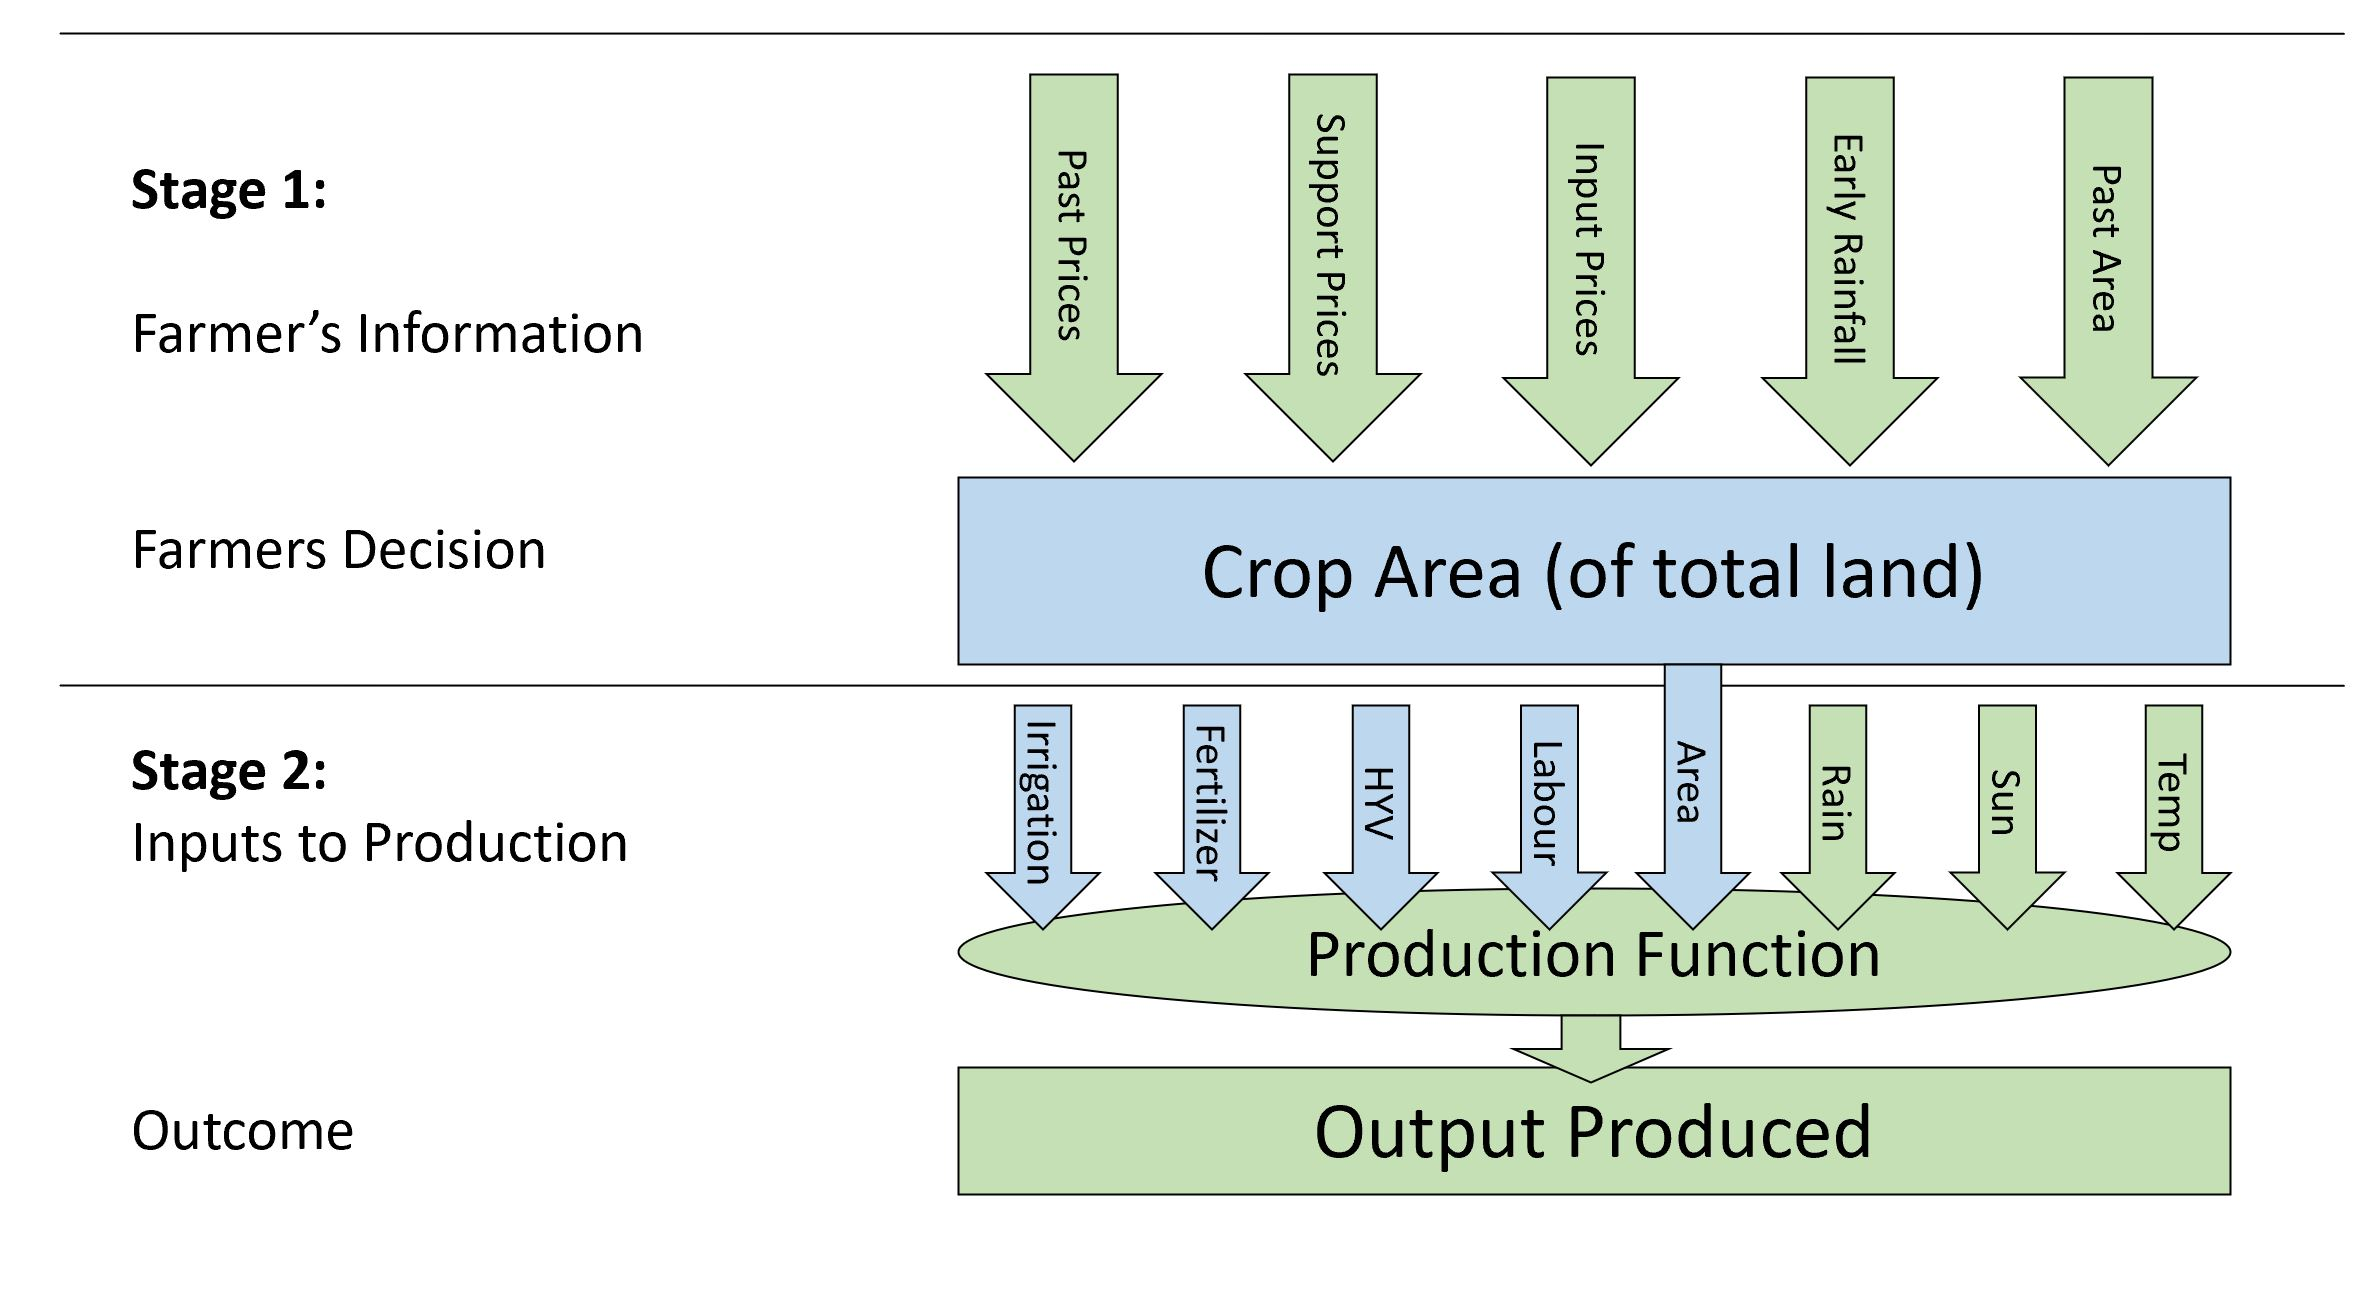
\includegraphics[scale=0.5]{fig_production_auffhammer.JPG}
    \caption{The farmer's problem.}
    \caption*{\footnotesize{\textit{Note:} At stage 1, the farmer observes relevant information, the realization of which is exogenous. Based on this, the farmer apportions some land for planting a given crop. In stage 2, inputs enter the production function (HYV = high yield variety). Inputs depicted by blue arrows are choice variables for the farmer, green ones are not. \\ \textit{Source:} Adapted from \citet{Auffhammer2014b}.}}
    \label{fig:production_auffhammer}
\end{figure}

Labour supply depends in many ways on all the other factors to fall in place first: No additional harvesters are needed if, for example, a drought wipes out your crops before they are ripe. It is this connection between the physical conditions for agriculture and the human labour inputs to it, which may prove helpful for exploring the more specific characteristics of child labour supply in that sector. 

One consequence of the complex nature-human interactions that characterise agricultural production is that the productivity of labour cannot be observed directly by the executive farmer, even if he were to monitor all workers constantly. Indirect measures of productivity, such as the number of tasks performed per worker, are also unavailable for most of the productive cycle: At harvest, one can judge the amount of produce harvested per worker and, at planting, the quantity of seeds sown or the area of land covered. Between planting and harvesting, however, labour productivity is not straight forward to measure indirectly as growth and crop quality are mostly determined by environmental factors. Since total production at the end of the harvest is a complex function of many worker's individual contributions and of the environment over time, individual workers' inputs cannot be easily disaggregated or compared. Thus an informational asymmetry arises. 

%Assuming that workers value leisure, the ex-post non-disaggregatability of total production means that they would like to freeride whenever they can knowing that the principal will be unable to detect their defecting behaviour. This moral hazard arises for all workers. For external wage labourers, the asymmetry is aggravated additionally by the fact that their wages are usually paid per week, day, or hour spent on the employing farm rather than by productivity units actually realised (remember that these are incommensurable most of the time). Avoiding work could be lucrative to the extent that there is still sufficient output at the end so that wages are paid and consumption needs are met. The employer only has one option to limit this behaviour, which is direct oversight. Overseeing labour becomes increasingly costly as farm size and labour force increase, yielding it unprofitable for most farms larger than a single plot \citep{Sen1981a}.

One result of this is the inverse relationship between a farm's size and its productivity, which was first noted in the case of India \citep{Sen1962} and has since been evidenced in LMICs across the world. The literature shows quite convincingly that - holding inputs constant - small family owned farms are more productive than bigger enterprises \citep{Sen1981a,Sen1981}. There is disagreement, however, on whether this is due to the lesser extent of moral hazard (e.g. shirking) among family members vis a vis wage workers\footnote{Household members have a direct interest in maximising farm output because their consumption is directly dependent on it. Wage workers, on the other hand, can benefit from defecting behaviour as long as output remains high enough so that a decline can credibly be attributed to solely environmental factors and wages continue to be paid.}, or due to the spatial dispersion of workers on bigger farms which drives up monitoring costs \citep{Sen1981a}. Either way, free-riding seems to be less of a problem on family-farms without labour market connections.

On the other hand, labour markets are crucial for insuring against crop failure. \citet{Kochar1999} presents evidence suggesting that the smoothness of household consumption in the presence of farm-specific crop income shocks reflects the ability of households to smooth income directly, by increasing their market hours of work. This is an early pointer to the important role that labour markets play in household consumption smoothing and, consequently, its effects on child labour allocation discussed in \citet{Dumas2015,Dumas2020}.

\subsection{Economic effects of climate change}
\label{sub:economic_effects_of_climate_change}

 Since child labour is not prominently featured as a topic in the ARE, the importance of this literature for the present study lies predominantly in providing a framework that can link climate and weather to socio-economic phenomena \textit{like} child labour.

Indeed, the relatively recent empirical literature on the economic impacts of climate change has turned the spotlight onto quantifying the effect of climate on many different socio-economic outcomes. Table \ref{tab:ARE_lit} gives a non-exhaustive list of such studies. Most of them report highly non-linear relationships between climate and the outcomes of interest \citep[e.g.][]{Schlenker2009,Burke2015}, and warm temperatures seem to be a particularly relevant factor for many climate responses \citep{Auffhammer2013}.

\begin{table}[t!]
    \singlespacing
    \centering
    \caption{Selected climate impact studies from ARE Economics.}
    \begin{tabular}{|p{2.8cm}|p{6cm}|p{2.2cm}|p{3.5cm}| }
    \hline
    & \raggedright\textbf{Paper} & \textbf{Climate Variables} & \textbf{Response\ \ \ \ \ \ Variable} \\
    \hline    
    \textbf{Agriculture} & \citet{Deschenes2007} & various & yields (HIC)\\
    \ \ & \citet{Mendelsohn2008} & various & yields (LMIC)\\
    \ \ & \citet{Schlenker2009} & various & yields (HIC)\\
    \ \ & \citet{Schlenker2010} & various & yields (SSA)\\
    \ \ & \citet{Welch2010} & various & yields (LMIC)\\
    \ \ & \citet{Lobell2011}& various & yields (globally)\\
    \ \ & \citet{Hertel2014} & various & yields (LMIC)\\
    \hline
    \textbf{Macro/Trade} & \citet{Barrios2010} & P & growth (SSA)\\
    \ \ & \citet{Jones2010} & T, P & exports\\
    \ \ & \citet{Burke2015}& various & aggregate output\\
    \ \ & \citet{Costinot2016} & various & trade advantage\\
    \ \ & \citet{Deryugina2017}& various & aggregate output\\
    \ \ & \citet{Dingel2019} & various & trade inequality\\
    \ \ & \citet{Burke2019}& various & aggregate output\\
    \ \ & \citet{Schlenker2019} & various & market outlook\\
    \hline
    \textbf{Migration} & \citet{Feng2010}& various & yields, migration\\
    \ \ & \citet{Marchiori2012}& various & migration (SSA)\\
    \ \ & \citet{Cattaneo2016}& T & migration\\
    \ \ & \citet{Missirian2017}& T & migration\\    
    \hline
    \textbf{Health} & \citet{Deschenes2014} & various & mortality rates\\
    \ \ & \citet{Isen2017} & T (in utero) & adult well being\\
    \ \ & \citet{Obradovich2017} & T & sleep\\
    \ \ & \citet{Burke2018} & T & suicide rates\\
    \ \ & \citet{Baylis2020} & T & temperament\\
    \hline
    \textbf{Warfare} & \citet{Hsiang2011} & various & conflict\\
    \ \ & \citet{Burke2015} & various & conflict\\
    \hline
    \textbf{Energy} & \citet{Auffhammer2014} & various & electricity demand\\
    \hline
    \end{tabular}
    \caption*{\footnotesize{\textit{Notes:} Studies by subject areas, denoting the type of climate variables used (P=precipitation, T=temperature, various) and the type of response variable for which the study controls. Location type (HIC = high income countries, LMIC = lower and middle income countries, SSA=Sub-Saharan Africa) provided where applicable. Note that climate variable types may indicate the use of more than one metric pertinent to that climate component (e.g. mean, maximum, minimum,...).\\ \textit{Source:} Author's own compilation.}}
    \label{tab:ARE_lit}
\end{table}

While the details differ, most of these papers roughly follow a two step procedure: first weather data is merged with data on the outcome of interest as well as some control variables. From this data set, a function describing the climate effect - called dose-response function or damage function - is estimated. The relevant coefficients are often estimated numerically due to the highly non-linear nature of climate effects. Once obtained, the dose-response function is used to project future effects of climate change. To this end, climate projections from a global climate model (GCM) are passed to the function. The function's output are then interpreted as the projected future values of the dependent variable.\footnote{This approach by itself has been dubbed the ``dumb farmer scenario'' \citep{Auffhammer2014a}, as it implicitly assumes that farmers continue business as usual despite climate change.}

The related methodological literature, in particular \citet{Timmins2009, Schlenker2010a, Auffhammer2013, Hansen2014, Auffhammer2018} and \citet{Hsiang2016a}, has developed a range of econometric strategies for estimating dose response functions, forecasting, and drawing climate insights from weather data. My empirical analysis in section \ref{sec:empirical_strategy} uses the framework of \citet{Hsiang2016a} in building a first bridge between this empirically driven literature from ARE and the aforementioned literature on child labour. Conceptually, rainfall, temperature, and other weather components are modelled to be jointly drawn from an underlying distribution which is commonly called `climate'. 

In order to model climate change and its effects, one must first define what exactly climate is. We never directly observe climate. What people perceive in their immediate environment is weather and it is weather, not climate, that has an immediate effect on their lives. Hermeneutics complicate this distinction further: humans learn from repeated experience, develop foresight, and adapt. As a result, weather can have direct and indirect effects. Direct effects of rain, for instance, include getting wet or losing harvest due to flooding. Analogous indirect effects are wearing a rain coat next time and installing a drainage system to safeguard crops. Thus, direct and indirect effects of weather are increasingly convoluted over time and space.

This distinction also exists, as immediate versus down-stream effects, in the Environmental Impact Assessment (EIA) literature \citep[see e.g.,][]{Noble2015}. Furthermore, EIAs distinguish between environmental changes and effects. Assuming that there is always some level of change in the ecosystem, environmental effects are then those additional changes induced by external shock to the system - the difference in differences. This broad conceptualisation of all environmental effects, transitory or persistent, neatly encompasses climate change.

The notion of human foresight about the weather is crucial as it suggests an implicit characterisation of climate as a probability distribution. While we may not exactly know ex ante what the weather will be at our position in a given future moment, we might have accumulated prior expectations about the `usual' extent to which precipitation, temperature, wind gusts, and other weather components tend to vary, about their typical transitory pace, and even about the approximate probabilities attached to each possible state conditional on the eventuated past and on the contemporaneous variance observed in other related weather components.

In developing such expectations, humans display an approximate understanding of the geophysical processes underlying the weather as they learn to appreciate the observable interdependence structure across weather components induced by these processes. Continuous observation of the weather is then equivalent to drawing independent random draws from an underlying distribution. As long as this distribution remains unaltered, the accuracy of one's expectations increases with the number of draws. Precipitation, for instance, differs by temperature and we intuitively expect snow when the temperature falls below zero degrees centigrade, but rain above that threshold. As long seasonal variation of temperature stays constant, this enables long-term planning of all kinds of economic activity in humans, as well as survival strategies in animals (e.g., hibernation) and plants (e.g., shedding foliage) more broadly. Equivalent long-term strategies occur everywhere on planet earth, always specifically geared towards the local climate.

Recent evidence from the United States shows that humans are surprisingly fast in correcting their expectations to account for climate change. The subjective baseline against which temperature is evaluated appears to be dominated by recent experience. In consequence, ``temperatures initially considered remarkable rapidly become unremarkable with repeated exposure over a roughly five year timescale'' \citep[][p. 4909]{Moore2019}. This rapid expectation adjustment relative to the pace of anthropogenic climate change has large implications for the notability of temperature anomalies as climate change progresses.\footnote{Notably, this attenuating presence-bias surrounding human perception of extreme weather may inhibit societal pressure for climate change mitigation efforts.} It also means that the two-fold effects of the static climate distribution - on effectuated weather and on people's expectations about it respectively - may carry over to the non-static setting with climatic change quite seamlessly. The following model is geared towards giving a first intuition as to what happens to child labour as climate change progresses. It is followed by an empirical exploration.

\section{Model}
\label{sec:model}

The model presented in this section draws from \citet{Jessoe2018}. Their model, in turn, is a version of the standard agricultural household model \citep{Singgh1986} with weather as an additional production factor \citep[as in][]{ravallion1988}. In this class of models, the household solves the production and consumption sides simultaneously, resembling their dual role as producers and consumers.

Two additional extensions are necessary in order to adapt this framework to the analysis of child labour. First, the household's aggregate utility function, which is left unspecified in 
\citet{Jessoe2018}, should exhibit child labour aversion in line with the luxury axiom \citep{Basu1998}. Secondly, the effective labour input $L$ must be disaggregated into child and adult labour. Furthermore, the functional form of adult-equivalent child labour units needs to be specified in order to accommodate complementarity and appropriately scale total time input according to the differences in productive capacity between child and adult labour time units. Following some preliminaries, I implement these extensions and solve the household's utility maximization problem.

\paragraph{Preliminaries:}
\label{sec:Preliminaries}
The ILO's International Programme on the Elimination of Child Labour (IPEC) defines child labour as

\begin{quote}
work that is mentally, physically, socially or morally dangerous and harmful to children; and that interferes with the children’s schooling by depriving them of the opportunity to attend school, either by obliging them to leave school prematurely, or by requiring them to attempt to combine school attendance with excessively long and heavy work \citep{ilo2021}.
\end{quote}
Because the various components of this definition are often hard to establish in practice, age is commonly used as a proxy by which to distinguish benign work from child labour. The ILO’s Convention No. 138 stipulates the relevant ages that different countries use to define child labour. In applied work, therefore, the age threshold needs to be adjusted to the relevant country context, with the upper limit at eighteen years in any case. In formulating a theoretical model, such an adjustable age threshold can be implemented on any household's age-ordering. Consider an agricultural household $\mathcal{I}=\{1,2,...,I\}$ whose $I>0$ members are ordered from youngest to oldest. Let $a_i$ be the age of household member $i\in\mathcal{I}$. Moreover, let $\underline{a}$ be the legal age at which an individual is no longer considered a child. Accordingly, $i$ is a child if $a_i<\underline{a}$ and an adult if $a_i\geq \underline{a}$. Let $\hat{\imath}$ denote the oldest child in the household. The household can, accordingly, be divided into $\hat{\imath}$ children and $I-\hat{\imath}$ adults.

Every member of the household is endowed with time, normalized at 1. By assumption, the $I-\hat{\imath}$ adults work all of the time, while the $\hat{\imath}$ children's time is divided between $e\in[0,1]$ time units of work effort on the household's farm and $(1-e)$ time units of non-work.\footnote{This non-work may involve going to school as well as leisure. This difference is of no consequence in this static setting. Of course, in an intertemporal maximization exercise - as part of a dynamic model - the consequences of deciding between education and leisure will have a tangible effect on the accumulation of human capital and associated earning capabilities.} For simplicity, the effort $e$ is assumed to be equal for all children.\footnote{While this assumption does not impact the model's implications, it considerably decreases the complexity involved in solving it. Some possible extensions - allowing for $e$ to vary across children - are discussed in annex \ref{app:time_allocation}.} Note that aggregate time endowment up to a given individual is equal to the number of individuals it has been aggregated over. For example, the aggregate time endowment of adults in $\mathcal{I}$ is $(I-\hat{\imath}$). 

\paragraph{Household preferences:}
\label{sec:hhpreferences}

Household $\mathcal{I}$ derives utility from the consumption of generic goods and services, which are denoted by $c$. Additionally, the household's decision makers are averse to child labour, as long subsistence consumption levels can be reached without it.

The following Stone-Geary utility function\footnote{This functional form is commonly used to model subsistence levels into expenditure systems. \citet{stone1954} first estimated the linear expenditure system associated with it and \citet{geary1950} was the first to derive it in theory, in a comment on earlier work by \citet{klein1947}. Therefore, it is also known as Klein-Rubin utility function.} with an additional child-leisure factor captures this trade-off \citep[cf.][]{Basu1998}.

\begin{equation}
\label{eq:UF}
    U(e,c)=(c-s)(1-e),
\end{equation}
where, $s$ is the subsistence level of consumption and the second term on the right hand side captures children's non-work. \citet{Basu1998} note that the specific form of this utility function implies ``that the child's leisure is a luxury good because doubling the household's wealth (from non-child-labour sources) leads to a more than doubling of child labour''(p. 420, footnote 11). This is the implementation of their luxury-axiom.

\paragraph{Labour equivalence:} Children tend to be less productive than adults. In agriculture, this stems from differences in physical strength, skill-refining experience, ability to manage equipment, and other productive traits - all of which favour adults.\footnote{The opposite is true when a productive activity requires specific characteristics that are more readily available in children. One particularly cruel example is mining in confined underground spaces, where children's small size allows for easier access and faster extraction of precious ores while minimising drilling costs  \citep[see e.g.][]{Odriscoll2017}.} It is common practice to multiply child labour with an adult-equivalence factor between 0 and 1, making it an imperfect substitute for adult labour \citep{Basu1998, Baland2000, Bhalotra2003, Basu2010, Dwibedi2017, Dumas2020}.\footnote{Similar household equivalence scales are commonly used in estimating household consumption systems, with children (the elderly) consuming a fraction (multiple) of adult consumption. For reference, see \citet{Pollak1979}, \citet{Lewbel1989}, \citet{Blundell1994}, \citet{Lewbel1997}, or \citet{Deaton1999}. While they are increasingly considered to be overly simplistic, equivalence scales are used in more involved methods, like the one presented by \citet{Dunbar2013}.}

In a similar fashion, let the full labour supply of household $\mathcal{I}$ be
\begin{equation}
    L=(I-\hat{\imath})+\gamma \hat{\imath}e,
\end{equation}
where the positive parameter $\gamma\in[0,1]$ defines the adult-equivalent productive capacity of child time allocated to farm work. That is, one child hour of farm work produces the same marginal returns as $\gamma$ ($<1$) hours of adult farm work. To further limit the model's complexity, this adult-equivalence parameter is assumed to be the same across children. Some possible extensions that allow it to vary by children's individual characteristics (e.g. age, sex, or prior work experience) as well as in relation to parental supervision are suggested in annex \ref{app:adult_supervision}.

\paragraph{Agricultural production:}
Agricultural goods are produced using labour $L$ and quasi-fixed land and capital $\bar{K}$. The quantity produced is given by $Q=f(L,\bar{K},\theta)$. As in \citet{ravallion1988}, the factor $\theta$ represents the realisation of weather, a higher value of which indicates weather that increases production. $f(\cdot)$ is a continuous and twice differentiable production function for which the following four inequalities hold:

\begin{equation}
\label{curvature}
    \frac{\partial f}{\partial L}>0, \quad \frac{\partial f}{\partial \theta}>0, \quad \frac{\partial^2 f}{\partial L^2}<0, \text{ and} \quad \frac{\partial^2 f}{\partial L \partial \theta}>0.
\end{equation}

\paragraph{Household problem:}

Household $\mathcal{I}$ is a price-taker in all markets. Formally, the household's problem is to maximise its utility, described in equation (\ref{eq:UF}), subject to its budget constraint
\begin{equation}
\label{eq:BudgetConstraint}
    (I-\hat{\imath})c+\hat{\imath}\beta c = f(L, \bar{K}, \theta),
\end{equation}
where $\beta\in[0,1]$ is the adult-equivalent of a child's consumption.

Note that this formulation builds on one more, rather strong assumption; the household is assumed to live in autarky, consuming the entirety of what it produces and nothing more or less. There are no functioning labour markets, where household members could either sell their own labour for wages or contract external labourers, nor consumer good markets for the household to trade its produce for money and supplement their consumption by buying externally provided goods and servies.

While assuming this extreme form of economic isolation may be warrented, to some extent, for subsistence farms in remote rural areas, it clearly does not hold for many other environments where children commonly work. The implications of labour, credit, and goods markets on child labour have been explored thoroughly in the literature \citep[see e.g.,][]{Baland2000, Bhalotra2003,Dumas2013, Dumas2015, Dumas2020}. I limit my analysis to the state of autarky and focus, instead, on the impacts of climate change.

Using Lagrange's method, and denoting the lagrangian multiplier as $\lambda$, the utility maximization problem yields the Lagrange function
\begin{equation}
\label{lagrange}
    \mathcal{L}(c,e,\lambda)=(c-s)(1-e) -\lambda \left[(I-\hat{\imath})c+\hat{\imath}\beta c - f(L,\bar{K},\theta)\right].
\end{equation}

The first order conditions, obtained by taking the partial derivative of $\mathcal{L}$ with respect to the three choice variables and setting them equal to zero, yield an exactly identified system of three equations with three unknowns. Solving this system for $c$ and $e$ gives the following identities.\footnote{This system can be solved either with pen and paper or on a computer. A python script for this purpose is available at \href{https://github.com/mathiasweidinger/MPPTH}{www.github.com/mathiasweidinger/MPPTH/}.}

\begin{equation}
\label{eq:consumption}
    c=\frac{f(L, \bar{K}, \theta)}{(I-\hat{\imath})+\beta \hat{\imath}}
\end{equation}

and

\begin{equation}
\label{eq:effort}
    e=1+\frac{s((I-\hat{\imath})+\beta \hat{\imath})+f(L,\bar{K},\theta)}{\gamma \hat{\imath} f'_L}.
\end{equation}
In equation (\ref{eq:effort}), the term $f'_L$  is a short hand for
\begin{equation*}
    \frac{\partial f(L,\bar{K},\theta)}{\partial L},
\end{equation*}
which is known to be strictly positive from the curvature assumptions formalised in equation (\ref{curvature}) above.

Equation (\ref{eq:consumption}) merely tells us that individual consumption is derived by dividing the households agricultural production by its member's adult-equivalent consumption needs. Equation (\ref{eq:effort}), on the other hand, shows that children's time effort working is increasing in the household's combined subsistence levels and in the household's production function. The fact that household production, itself, increases in weather means that a weather shock directly affects child labour supply. The direction of this effect on $e$ depends on the sign of the cross-derivative of output with respect to labor and weather.

In other words, child labour effort increases with weather that is ``good'' for production and decreases with weather that is ``bad'' for it. This means that no one variable's effect should be expected to be monotone; either consistently positive or negative. Rather, very low or high levels of precipitation or temperature will have negative effects on plant growth and, thus, on production while temparate weather should facilitate plant growth and enable production. For instance, rain is generally conducive to production but floods or droughts are not.

In terms of climate change, this would suggest that the direction of a sustained shift in weather patterns would also indicate the direction of the resulting shift in child labour. If, as most projections suggest, climate change has adverse effects on agricultural productivity, this result projects a decrease in child labour as a result of climate change.

Of course, the omission of labour markets strongly limits the real life relevance of this model. While negative weather shocks tend to lead to a lesser harvest and, thus, to less labour demand during that stage of production, it is not at all clear wether this will result in more or less child labour. Likely, a sustained decrease in production would have an income effect which, over time, could make it prohibitively expensive to contract external labour for harvesting, sowing, and other activities. If that is the case, the effect of climate change may well be more child labour.

The next section investigates empirically the effect of climate change on child labour in the case of Nigeria. Negative climate coefficients\footnote{In the sense that coefficients should be negative for those variables, which are expected to have a negative effects on the agricultural production function.} would indicate that the model above is useful in explaining child labour supply in subsistence agriculture. In the opposite case, labour-market effects - which are omitted above - may be dominant.

%%%%%%%%%%%%%%%%%%%%%%%%%%%%%%%%%%%%%%%%%%%%%
%%%%%%%%%%%%%%%%%%%%%%%%%%%%%%%%%%%%%%%%%%%%%
%%%%%%%%%%%%%%%%%%%%%%%%%%%%%%%%%%%%%%%%%%%%%


\section{Case selection and data processing}
\label{sec:case_selection}

Nigeria is the most populous and the sixth-most densely populated country in Africa\footnote{With a population of 200 million, Nigeria is also the sixth-most populous country in the world.}, and its 2020 nominal GDP of USD $450$ billion makes it the biggest economy on the continent \citep{WorldBank2021}.\footnote{In terms of purchasing power parity, only Egypt narrowly outperforms Nigeria.} About half of the population live in urban areas, particularly the large metropolitan areas in the South and Southwest towards the country's coast on the Gulf of Guinea. Moving North, the population density decreases gradually, giving way to wide savannahs and steppes which are characterised predominantly by agriculture.

Nigeria exhibits some characteristics which make it a particularly well-suited case study in the context of this paper. First, while exact estimates are hard to come by, it is generally acknowledged that child labour is rampant. The \citet{USDepartmentofLabor2021} estimates that 13 million children work on a regular basis. In May 2019, the ILO's Country Office Director stated publicly that at least 43 percent of Nigerian children - 15 million - were trapped in forced, largely unpaid labour \citep{ILO2019}. This is double the SSA average, which itself is the highest regional average in the world. While child work is also common in other sectors, such as domestic servitude or gold mining, the vast majority of working children are employed on their families' farms.

Second, Nigeria exhibits high levels of (rural) poverty and socio-economic inequality. Although it is one of the fastest-growing countries in the world, almost half of its population still grapples with extreme poverty. With a Gini index of 35, income inequality lies close to the SSA average. This shows a highly uneven distribution of wealth between many poor and very few rich households. According to the most recent national report, 40 percent of the total population, or almost 83 million people, lived below the country's poverty line of 137,439 Naira (USD 381.75) per person per year. While most wealth is located in the big metropolitan areas such as Lagos, Ibadan, and Abuja, poverty is both more prevalent and deeper in rural areas, where the headcount is above 50 percent and the poverty gap amounts to 17.4 percent of the poverty line on average in contrast to the four percent observed in urban areas \citep{NBS2020}.

The simultaneous concentration of (extreme) poverty and rampant child labour in rural areas closely resembles two key assumptions of the model derived in section \ref{sec:model}: the luxury axiom, expressed by the subsistence terms in the Stone-Geary utility function, operationalises the assumption that poverty is the principle driver of child labour. The agricultural focus of most households' economic activity further suggests that a large enough subpopulation engages in \textit{agricultural} child labour specifically. Taken together, these facts mean that Nigeria provides a highly relevant and suitable case to study empirically.

\subsection{Climate and agriculture in Nigeria}

Nigeria's climate can be divided into two main seasons: ``dry winter from November to March, and rainy summer from April to October''\citep[][p. 61]{shiru2019}. Beyond seasonality, Nigeria's climate is characterised by differences in humidity, which varies by latitude as shown in figure \ref{fig:climatezones}. The country's northernmost fifth is covered by arid steppe and desert (red and yellow), whereas the remaining southern portion displays a humid tropical climate (shades of blue); savannahs in the center and some monsoon and rainforest climates in the southernmost regions. 

\begin{figure}[h!]
    \centering
    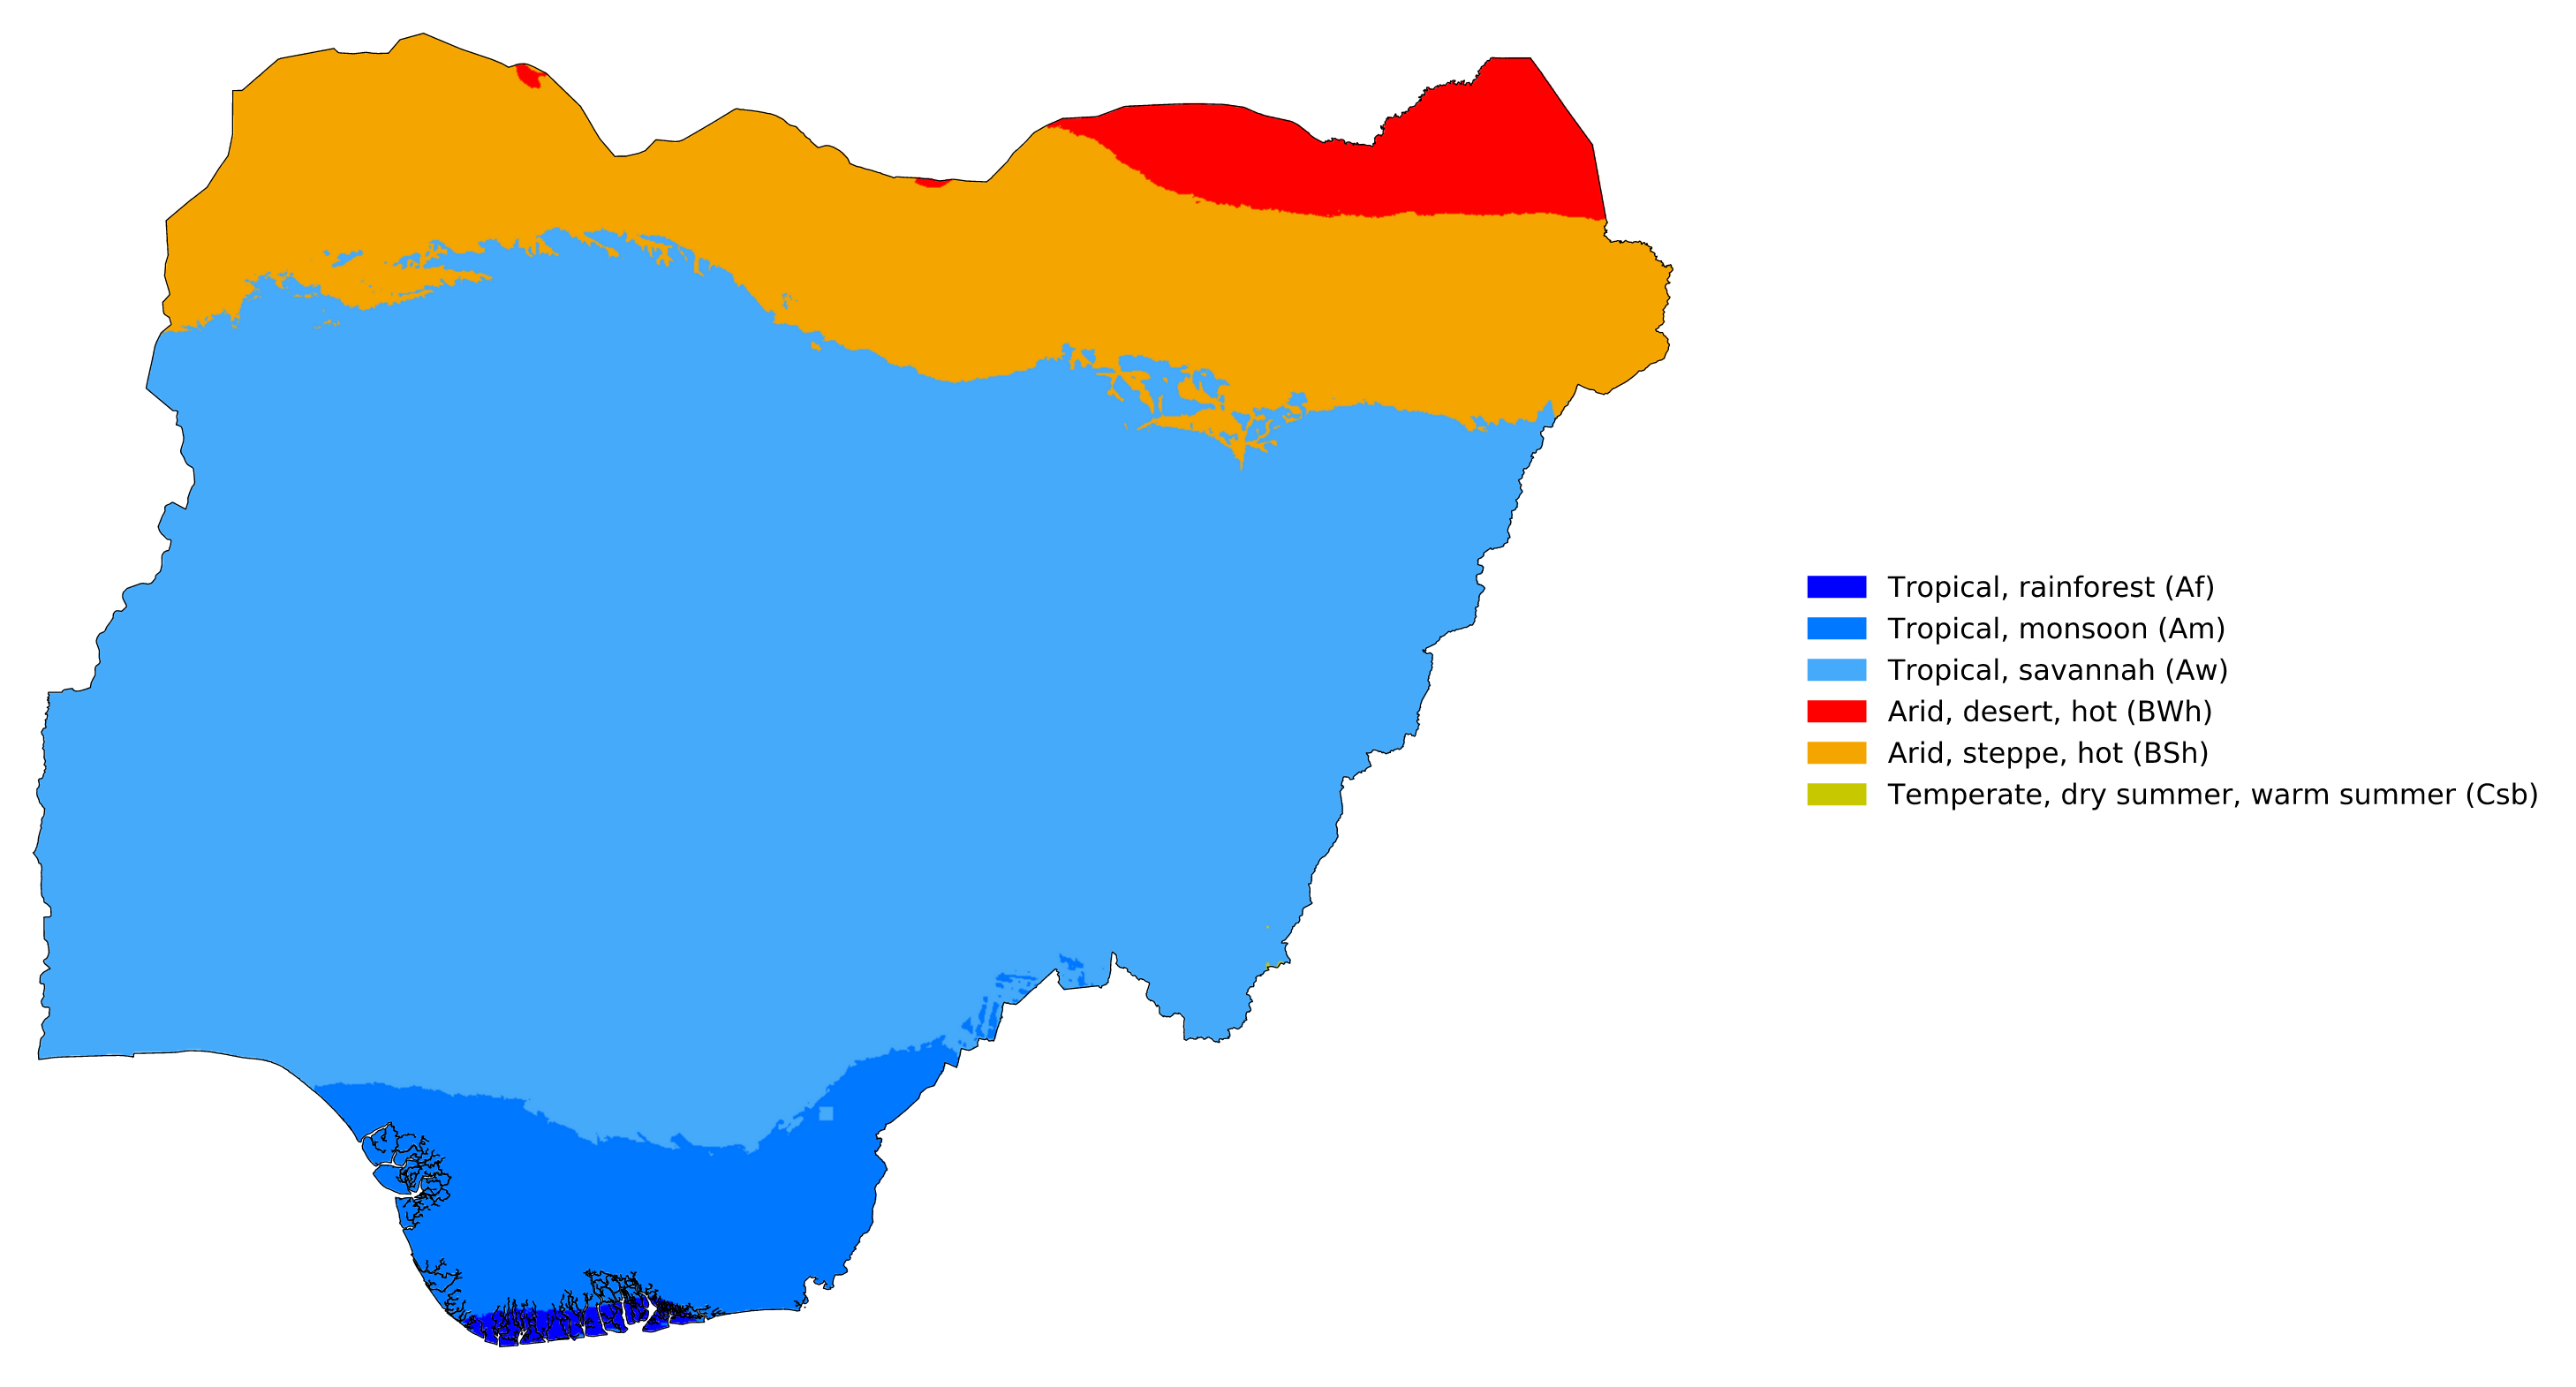
\includegraphics[scale=0.33]{../outputs/climatezones.png}
    \caption{Climate zones of Nigeria.}
    \caption*{\footnotesize{\textit{Notes:} Köppen-geiger climate classification at 1-km resolution. \textit{Source:} \citet{Beck2018}.}}
    \label{fig:climatezones}
\end{figure}

Partly on account of its geography, Nigeria produces a wide variety of crops. Data shows that most farmers ``are involved in more than one agriultural activity, even though at varying degrees" \citep[][p. 99]{naerls2015}. At 99.1 percent of surveyed farmers, however, virtually every agricultural household grows at least some food crops for household consumption, whereas only 52 percent reported growing cash crops. This statistic emphasizes the role of subsistence agriculture in providing food security across the country.

Agriculture varies regionally, closely tracing the climatic differences outlined above. The most important food crops include Corn, Sorghum, Millet, Rice, Cassava, Yam, Cocoyam, Groundnut, Cowpea, and Soybean. The drier northern areas mostly produce cereals and variety of crops increases southwards. While some crops are confined to particular climates, others are grown across the spectrum. \citet{shiru2019} study the distribution of several crops across Nigeria's climate zones and note that, while both Corn and Rice are grown throughout the country,
their growing season in the North differs from that in the South. This is perhaps best explained by the seasonality of rainfall in the otherwise dry Northern regions. In total, \citet{shiru2019} provide an approximate calendar of cropping seasons for five crops, which gives insight into the yearly agricultural cycle from sowing, thru growing, to harvesting (see figure \ref{fig:growingseason} below). Yams total a growing season of up to eleven months, being planted as early as February thru April and harvested as late as October thru December. Millet, which only grows for five months (May to September) at most, has the shortest growing season, closely followed by corn. January is the only month during which the agricultural cycle lays completely dormant; the last harvests seize in December and planting starts in late February and becomes more frequent throughout March, April and May.

This brief overview of the climatic and agricultural characteristics of Nigeria provides the necessary context for the data that I introduce next. The extent of the growing seasons, for instance, informs the temporal units of the panel data used in the analysis and dictates how to process relevant climate variables. The following section discusses the sources of this data and how they were selected.

\subsection{Data sources}
\label{sub:data_sources}
Analysing the prevalence of child labour as a function of climate change must involve at least two types of data: weather observations and individual-level work data for children. In order to control for possible confounders, other individual and household characteristics should be added. A last and absolutely vital requirement is, of course, that all these data are geo-coded in accordance with a coordinate reference system (usually degrees of latitude and longitude) so that they can be matched. This study relies on two data sources to meet these requirements.

First, the individual and household variables are provided by the Nigeria General Household Survey (GHS), which is part of the World Bank's Living Standards Measurement Surveys (LSMS) programme and is conducted by Nigeria's National Bureau of Statistics in collaboration with Nigeria's Federal Ministry of Agriculture and Rural Development, the National Food Reserve Agency, the Bill and Melinda Gates Foundation and the World Bank. GHS is an ongoing long-term project to create a growing panel of agricultural and household data in such a way as to allow the study of agriculture’s role in household welfare over time. It collects information on household agricultural activities along with other information on the households like human capital, other economic activities, and access to services and resources.

The GHS-Panel lends itself extremely well to this paper's research question thanks to its succinctly agricultural focus. To date, the survey instrument has produced four waves (2010-2011, 2012-2013, 2015-2016, 2018-2019), the first three of which are used in this analysis. The decision to omit the most recent wave in this analysis was taken due to what seems to be non-random attrition of households after wave 3, concentrated in rural areas. Each wave of the GHS-Panel is a cross-section of approximately 22,000 individuals in approximately 5,000 households which are representative of the Nigerian population at large. Each GHS wave consists of two visits, one at the end of the planting season, between September and November, and the other at the end of the harvest, February thru April of the following year. Thus, the final panel consists of six, approximately biannual cross sections.

The most relevant parts of the GHS panel are the individuals' labour information (e.g., hours worked, wages earned, sectoral information, and time spent on household chores), agricultural plot and production information by household, as well as the more general socio-economic standing of the households and their individual members. This includes education, which is of particular interest as it may compete with child labour for children's time allocation. Apart from its agricultural focus, what sets the GHS apart is the decision by its creators to include approximate spatial coordinates of the enumeration areas (EA) where the households are located.\footnote{EAs are the smallest geographical partition present in the GHS, approximately equivalent to a community or a cluster of villages. Other, higher order units are equivalent to Nigeria's administrative divisions of Legislative Government Areas (LGA), provinces, and regions.} This allows users to spatialise the dataset and combine it with other data sources according to the coordinates attached.

I spatialise the GHS panel dataset and combine it with climate data. Version 4.05 of CRU TS (Climatic Research Unit gridded Time Series) is a widely used global climate dataset. It is derived by the interpolation of monthly climate anomalies from extensive networks of weather station observations.\footnote{For detail on how CRU TS was constructed, see the accompanying publication \citep{harris2020}.} CRU TS 4.05 includes ten timeseries of geophysical variables that jointly depict the development of the world's climate at a monthly interval. This data, which is available from January 1901 to December 2020, is laid out on a 0.5° latitude by 0.5° longitude grid (approximately 50 kilometres by 50 kilometres cells) across all major land masses (except Antarctica). This high resolution allows capturing a great part of cross-community climate variation between EAs.

\subsection{Variables}
\label{sub:variables}

This section describes the main variables used in the analysis and how they were constructed.

\subsubsection{GHS variables}
\label{subsub:ghsvars}
The survey recorded the ``hours worked last week in a job'', as well as the ``minutes spent on chores yesterday''. In order to streamline the time-frame of these two variables, the hours worked in a job are divided by seven and the minutes spent on chores are divided by sixty. Adding up the two results for every individual gives their daily work hours including chores.\footnote{Note that this often yields non-integer values due to the conversion of the chore variables from minutes to hours. Moreover, this construction relies on the assumptions that (i) last week's workload is representative for the overall workload, and (ii) that yesterday's chore minutes are representative of every day's time spent on chores.} Lastly, I filter the variable by age and set it to missing for individuals aged 18 or above. The final result is an approximate measure of daily hours spent in child labour including chores.\footnote{Alternative measures can be obtained, for instance by omitting the chores component or by filtering out observations outside the agricultural sector. All these alternative measures turn out to be virtually equivalent with correlations among them and the original variable ranging between $0.92$ and $1$. Since the additional constraints do, however, cost observations I proceed with the initially proposed variable.} Other variables which are taken more or less unaltered from the GHS-panel\footnote{In some cases, they were recoded to subsume many categories into one or to facilitate interpretation of results.} are household consumption, household size, sex, and age.

To assess the welfare of a given household, a multidimensional poverty index (MPI) is constructed, closely following the approach spearheaded by \citet{alkire2011} and most recently applied globally in \citet{alkire2020}. I try to retain the same dimensions, indicators, and relative weights used in \citet{alkire2018, alkire2020}, subject to data availability in the GHS. Each of the indicators used is related explicitly to one or more of the SDGs.\footnote{For a recent application to the SDGs, see the joint publication by \citet{ophi2020}.} Multidimensional indices are particularly attractive because they can be disaggregated \citep{bourguignon2003, foster1984}, in addition to fulfilling the properties usually required by poverty metrics \citep[see][]{Sen1976}.\footnote{For a critical review of the MPI literature, see \citet{ravallion2011}.}

The health dimension is comprised of two indicators. Nutrition, which is related to SDG 2 ``Zero Hunger'', codes a household as deprived if there was a situation in the last 12 months when there was not enough food to feed the household members. Child mortality is measured by the number of male and female children, born to women between 12 and 49, who died in the household. If this number is, on average across the household's eligible females, 1 or greater the household codes as deprived. Child mortality relates directly to SDG 3 ``Health and Wellbeing". Both measures are equally weighted 1/6 each so that health accounts for a third of the MPI. 

The education dimension also consists of two indicators. Years of schooling codes a household as deprived if no eligible household member has completed six years of schooling. Second, a household is deprived in terms of school attendance if any of its school-aged children is not attending school at the age-appropriate level up to class eight. Both education indicators are clearly related to SDG 4 ``Quality Education". Again, each of the education indicators is weighted 1/6, giving education a total weight of 1/3.

The last dimension of poverty is living standards, measured by six variables which are each weighted 1/18. A household is deprived in cooking fuel, if it cooks using solid fuel such as dung, agricultural crop, shrubs, wood, charcoal, or coal. In terms of electricity, a household is deprived if it has no electricity in the home. Both cooking fuel and electricity are central to SDG 7 ``Affordable and Clean Energy''. Sanitation deprivation occurs if a household has no or only an unimproved sanitation facility, or if it has an improved facility but shared with another household. A household is coded as deprived of drinking water if its source of drinking water is not safe for human consumption or if safe drinking water is 30 minutes or longer away by foot (round trip). Both sanitation and drinking water are basic needs acknowledged in SDG 6 ``Clean Water and Sanitation".

In relation to SDG 11 ``Sustainable Cities and Communities'', a household is deprived in housing if it has inadequate housing materials in any of the three components floor, roof, or walls. Lastly, a household is considered asset deprived if it does not own more than five of the these: sofa, chairs, table, mattress, bed, mat, sewing machine, gas cooker, electric stove, gas stove, kerosene stove, fridge, freezer, air conditioner, washing machine, electric clothes dryer, bicycle, motorbike, car or other vehicle, generator, fan, radio, cassette recorder, Hi-Fi sound system, microwave oven, iron, television set, computer, DVD player, satellite dish, and musical instrument. The indicator of asset deprivation is related to SDG 1 ``No Poverty''.

\subsubsection{Climate variables}
\label{subsub:climatevars}

The ten different geophysical variables of CRU-TS can be further categorised as primary, secondary, and derived variables. Primary variables are those that are directly measured at ground station level and have no synthetic component. They are mean temperature over two months (TMP), diurnal temperature range over two months (DTR), and the precipitation rate (PRE).

Secondary variables differ from primary variables in that they have fewer direct observations available. The synthetic estimates are estimated using empirical relationships with the primary variables. Vapour pressure (VAP) is generated from TMP, and DTR as described in \citet{harris2020}. The count of wet days (WET) is defined as the number of days in a month on which PRE $\geq0.1$ millimetres - a metric used in diverse areas including evaluation of satellite observations and of potential evapotranspiration equations. It is compiled using the same interpolation algorithm as in \citet{harris2014}. Synthetic cloud cover observations (CLD) are computed from DTR as in \citet{harris2014}, using station-based values. CLD is the percentage of cloud coverage averaged over the month.

Derived variables are entirely synthetic as their values are imputed from the observed values using empirically validated formulae. Minimum and Maximum temperature over two months (TMN and TMX) are derived arithmetically from TMP and DTR as described in \citet{harris2014}. Both are useful metrics, for instance for monitoring droughts, agronomic production and river basin vegetation. Freezing days per month (FRS) is the number of days in a month that record TMN $\leq 0$ degree Celsius. It is derived from TMN using an empirically determined function and is commonly used in dendroclimatology and health. Lastly, potential evapotranspiration (PET) is calculated from TMP, VAP, and CLD using the Penman-Monteith formula \citep{allen1998}, the United Nations Food and Agriculture Organization's (FAO) standard method for modelling evapotranspiration, as explained in \citet[][pp. 1071 - 1072]{ekstrom2007}. PET is defined as the amount of evaporation from the ground into the atmosphere that would occur if a sufficient water source were available. It is an important variable with regards to agriculture as it directly affects plant growth. If PET exceeds PRE, a place is considered dryland.

Table \ref{tab:cruvars} shows the variables of CRU TS, their units and their correlation decay distances (CDDs). A variable's CDD is defined as the distance where the correlation between one station and all other stations decays below $1/e$. The search radius for the selection of stations for the interpolation in CRU TS is set equal to the CDD as this optimises accuracy \citep{harris2020}. In other words, CDD is the distance between a station and a grid cell beyond which a station's raw observations are not useful for interpolating the climate variable at the cell. Generally speaking, precipitation has a rather low CDD as it is highly spatially concentrated, whereas temperature and vapour pressure usually vary over greater distances.

\begin{table}[t!]
    \singlespacing
    \centering
    \caption{CRU TS variables.}
    \begin{tabular}{|p{6cm}|p{1cm}|p{3cm}|p{2cm}| }
    \hline
    \raggedright\textbf{Variables} & \textbf{Code} & \textbf{Units} & \textbf{CDD(km)} \\
    \hline    
    \textbf{Primary} & \ \ & \ \ & \ \ \\
    \quad Mean 2m temperature & TMP & degrees Celsius & 1200\\
    \quad Diurnal 2m temperature range & DTR & degrees Celsius & 750 \\
    \quad Precipitation rate & PRE & mm/month & 450 \\
    \textbf{Secondary} & \ \ & \ \ & \ \ \\
    \quad Vapour pressure & VAP & hPA & 1000 \\
    \quad Wet days & WET & days/month & 450 \\
    \quad Cloud cover & CLD & percentage & 600 \\
    \textbf{Derived} & \ \ & \ \ & \ \ \\
    \quad Frost days &FRS& days/month & 750 \\
    \quad Minimum 2m temperature &TMN& degrees Celsius & 1200 \\
    \quad Maximum 2m temperature &TMX& degrees Celsius & 1200 \\
    \quad Potential evapotranspiration &PET& mm/day & n/a \\
    \hline
    \end{tabular}
    \caption*{\footnotesize{\textit{Notes:} A wet day is one receiving $\geq 0.1$ mm precipitation. Minimum and maximum temperatures are the monthly means of the individual daily minimum and maximum temperatures; they are not the overall minimum or maximum temperature recorded each month.\\ \textit{Source:} Adapted from \citet{harris2020}.}}
    \label{tab:cruvars}
\end{table}

\subsection{Point value extraction from the 2D grid}
\label{sub:combining}

The spatial scale of the CRU-TS data is laid out on a grid of 0.5 by 0.5 degrees according to the standard (viz. longitude and latitude) coordinate reference system. That means that CRU-TS has two-dimensional spatiality. The GHS data, on the other hand, is made up of observations at distinct (one-dimensional) points on the same standard coordinate reference system. These geo-code the location of the households present in GHS. For each of these locations, a one-dimensional value needs to be extracted from the two-dimensional CRU-TS grid.

For every EA in the GHS dataset, I compute the location-specific timeseries for every climate variable in CRU TS 4.05. To smoothen transitionary differences between climate cells, every EA's climate variables are obtained by taking a weighted average of all the (two-dimensional) cells which fall within a circular buffer of, for instance, 20 kilometres around the (one-dimensional) EA's centroid coordinates. This computation increases the accuracy of the climate data further, mirroring the resolution of EAs by averaging over two or more cells. Therefore, depending on the length of the circle's radius and the resolution of the climate grid, the climate variable's value at the EA coordinates is the weighted mean of one or more grid cells' values.\footnote{It is not necessary to weigh this sum by CDD, because the radius of the buffer should be smaller than any variable's CDD by an order of magnitude.} 

\begin{figure}
    \centering
    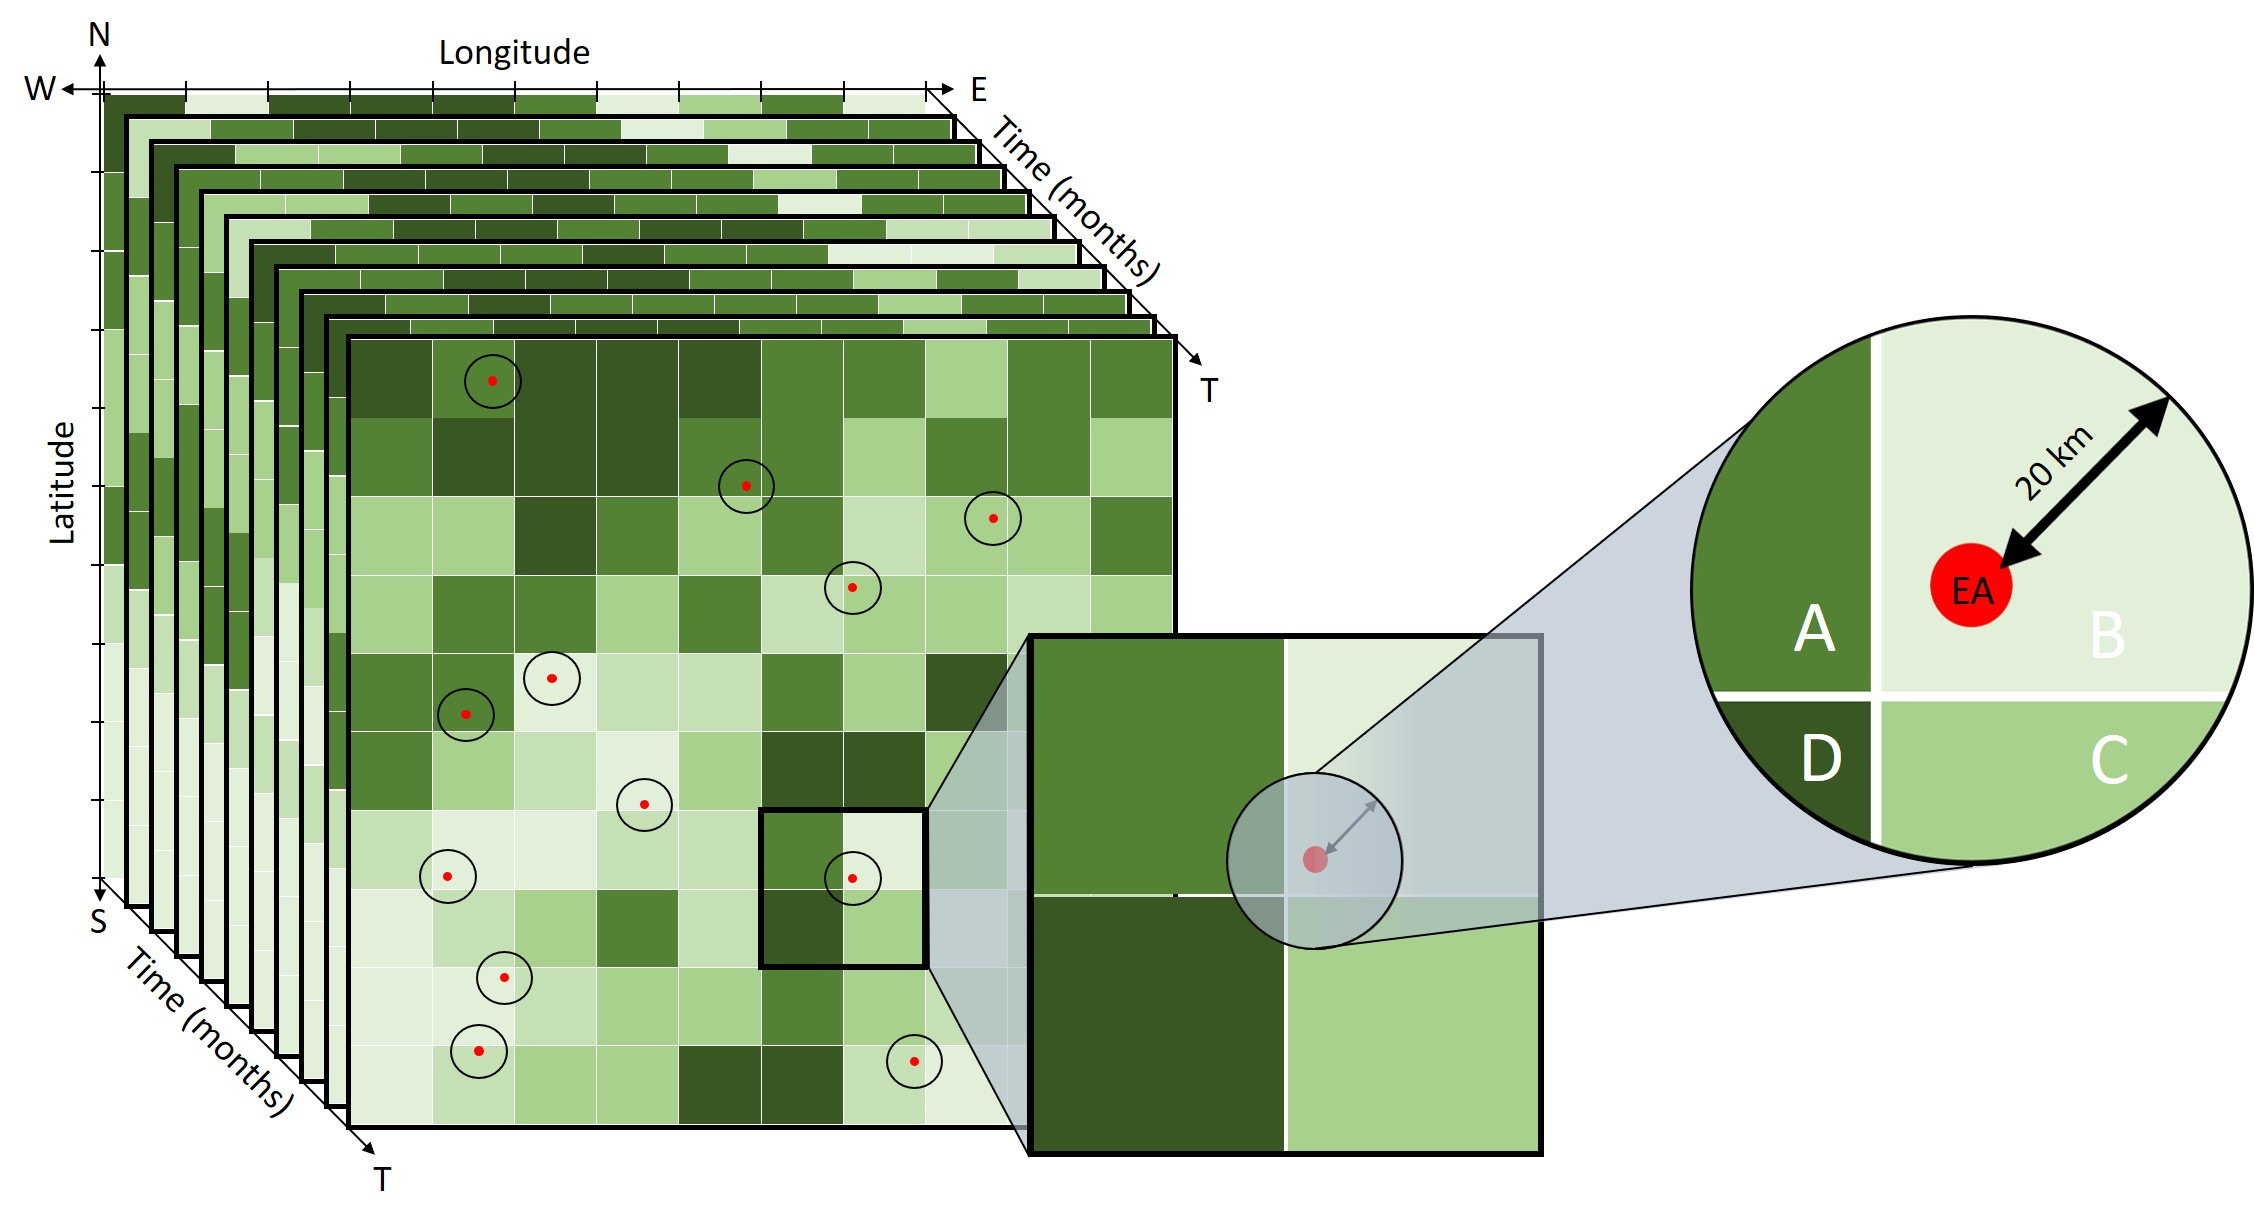
\includegraphics[scale=0.33]{../outputs/buffer.JPG}
    \caption{Smoothing climate variables using a circular buffer}
    \caption*{\footnotesize{\textit{Note:} Time series of climate variables take the form of three dimensional ``stack'' of coordinate grids, one for each timepoint. Each of these grids is composed of cells. Every cell, in turn, holds the measured value of the variable within its spatial limits at the grid's time point. The three dimensional grid stack on the left has the following axes: latitude from North (N) to South (S), longitude from West (W) to East(E), and discrete time in monthly intervals (T). Every grid's cells are coloured in shades of green that indicate the value of the climate variable on a continuous scale (e.g. monthly mean temperature in degrees celsius). The red dots represent the EA locations from the spatialised GHS data. Around every EA centroid, a circular buffer with radius $r=20$ kilometres is drawn. The exact value at the EA's location is then imputed by taking the weighted average of the cell segments (in order of size) B, A, C, and D that fall within the buffer, weighted by their respective surface areas. \\ \textit{Source:} Author's own compilation.}}
    \label{fig:buffer}
\end{figure}

To consider this formally, let a circle with radius $r_{it}$ be drawn around a household $i$'s position on each temporal layer grid $t = \{1, 2, 3,\dots, T\}$.\footnote{The midpoint circle algorithm is one of many digital circle generation algorithms that can be used to determine the points needed for rasterizing such a circular buffer \citep[see, e.g.,][]{barrera2016}.} Let $A_{it}$ be the total area enclosed by said circle. Let $n_{it} =\{1,2,\dots,N_{it}\}$ denote the $N_{it}$ grid cells which fall, at least partly, within the circle's area $A_{it}$. Each $n_{it}$'s portion within the circle has an area of $a(n_{it})\leq A_{it}$. Moreover, write the climate in grid cell $n_{it}$ as $c(n_{it})$. Now the value of the climate variable at household $i$ during time $t$ is approximated by

\begin{equation}
    c_{it}\approx \sum_{n_{it}=1}^{N_{it}}\frac{a(n_{it})}{A_{it}} c(n_{it}).
\end{equation}


Figure \ref{fig:buffer} is a schematic representation of this procedure as applied to the data. I chose a radius of 20 kilometres for the circular buffer, which is far enough to allow for mixing of different grid cells, but lies well within the variables' CDDs. As there are no missing values in CRU TS, ten full monthly time series (one per variable), covering 1999-2020, can be created for each household.\footnote{For implementing this in the R statistical programming language, see the \texttt{buffer} option of the \texttt{extract} command from the \texttt{R}-library \href{https://cran.r-project.org/web/packages/raster}{\texttt{raster}} \citep{hijmans2020} and its successor \href{https://cran.r-project.org/web/packages/terra}{\texttt{terra}} \citep{hijmans2021}.}

\section{Econometric strategy}
\label{sec:empirical_strategy}

To identify the causal effect of climate on child labour hours, \citet{Hsiang2016a} prescribes that a panel data model with fixed effects (FE) is needed, as it accounts for unobserved, time-invariant variables. The regression in question can be represented by the usual linear, unobserved effects model \citep[see e.g.,][]{wooldridge2010}: for any child $i$ and time $t$,
\begin{equation}
\label{eq:linear_FE}
    y_{it} = \alpha_i + \mathbf{c}_{i\tau}\beta + \mathbf{x}_{it}\gamma + \varepsilon_{it},
\end{equation}
where $\mathbf{c}_{it}$ is the vector of climate variables and $\beta$ is the vector that includes the coefficients of interest. Moreover, $\mathbf{x}_{it}$ includes control variables at the individual and household level, the effects of which are captured by the vector $\gamma$. $\alpha_i$ denotes the unit-specific fixed effects and absorbs the effects of time-invariant factors, including unobservables. Lastly, $\varepsilon_{it}$ is the idiosyncratic error term.

\citet{huntington1922} was perhaps first to note that this approach lends itself to estimating climate effects. In Equation \ref{eq:linear_FE}, the climate variables are taken to be observed at the same time intervals $t$ as child labour. However, the CRU-TS data is recorded monthly, whereas child labour (like all other GHS variables) occurs biannually. The next paragraphs closely trace \citet{Hsiang2016a} in recovering instantaneous effects from coarser data. They also extend the flexibility of the estimated climate effects.

\subsection{Recovering local and instantaneous non-linear effects}

The existing literature suggests that there is some value in letting the climate variables enter the regression using a flexible functional form. This flexibility is justified for the following reasons: first, prior work estimating the effects of climate metrics has documented important non-linearities across a wide array of responses \citep{Carleton2016} such as excess mortality from heat days \citep{deschenes2011} or crop yield damage from heat hours\citep{Schlenker2009}; second, an appropriate flexible functional form should reveal the shape of the underlying response function, linear or otherwise \citep{Hsiang2016a}; and third, it makes intuitive sense that plant-growth - the yield of which constitutes the physical output of household production - exhibits an optimal set of climate inputs, below or above which growth will be less than optimal. In fact, agricultural experiments show ``that below (and above) certain thresholds, plants cannot absorb (additional) heat, while within the bounds of an upper and lower threshold heat absorption increases linearly with temperature''\citep[][p. 239]{Jessoe2018}. Thus, agronomic studies suggest that accumulated exposure to heat over the growing season, rather than seasonal averages, determine crop growth. This also strongly suggests that responses are non-linear.

Following the approach presented in \citet{Hsiang2016a}, let the instantaneous non-linear effect of climate for a household $i$ in month $\tau$ be $f(\mathbf{c}_{i\tau})$, and let this function be approximated as a linear combination of $M$ simple non-linear functions, so that

\begin{equation}
\label{eq:nonlinear_approx}
    f(\mathbf{c}_{i\tau})\approx \beta_1 f_1(\mathbf{c}_{i\tau}) + \beta_2 f_2(\mathbf{c}_{i\tau})+\dots+\beta_M f_M(\mathbf{c}_{i\tau}) = \sum_{m=1}^M \beta_m f_m(\mathbf{c}_{i\tau}),
\end{equation}
where $\beta_m$ are constant coefficients. 

One common approach to model these non-linear responses is to fit $M$ polynomials to the data. However, polynomials of degrees higher than three are not straight-forward to interpret.\footnote{A linear model represents a system with a constant rate of change, a quadratic model a system with a rate of change that increases or decreases at a fixed rate (the acceleration), and a cubic model represents a system in which the acceleration changes at a constant rate. Similar correspondences do not exist for higher order polynomials.} An alternative to increasing the degree of the fitted polynomial to account for curvature is to divide the range of the data into smaller pieces and apply polynomials of lesser degree to each of the subintervals, stipulating that the resulting function be continuous \citep[see e.g.][pp. 275- 279]{greene2018}. However, the use of such truncated polynomials can sometimes lead to numerical problems.\footnote{If two knots are very close then the associated truncated polynomial terms will be very similar for all observations, almost co-linear, and the fitting algorithm will become unstable. Additionally, the values in the design matrix can be very large which can lead to overflow errors \citep[see e.g.,][]{hastie2009a}.} These problems can be avoided in practice by using a different set of functions in place of the truncated polynomials.

There exist several sets of functions which produce the same range of fitted curves, called equivalent bases \citep{hastie1987,hastie2009a}. One commonly used variant are B-splines.\footnote{Although any function that can be fit with the truncated polynomials can also be fit with B-splines, and vice versa, the B-spline basis functions are not colinear making the computational algorithms for fitting splines much more stable.} I use a natural cubic B-spline with knots at equally spaced interior points to achieve a flexible functional form. The spline divides the climate variables into five bins (i.e. $M=5$) according to the data's percentiles and fits the equivalent of a cubic function to each segment. This offers a non-linear alternative to using the climate data as is.\footnote{This and other approaches to model non-linearity are considered in more detail by \citet[][p. 18-19]{Hsiang2016a}.}

To address the difference in frequency between the GHS and CRU-TS data, let $\tau$ as used above denote the monthly interval of the CRU-TS data and write the biannual GHS frequencies as $t$. Assuming that the outome of interest is a linear sum of $f(\cdot)$ across points in time (i.e., temporal separability), the regression in Equation \ref{eq:linear_FE} can be rewritten as 

\begin{equation}
    y_{it}=\alpha_i+\left[\sum_{\tau\in t}f(\mathbf{c}_{i\tau})\right] + \mathbf{x}_{it}\gamma + \varepsilon_{it}.
\end{equation}
Substituting the approximation from Equation \ref{eq:nonlinear_approx}, this becomes

\begin{equation}
    \label{eq:combination}
    y_{it}\approx\alpha_i + \sum_{m=1}^M \beta_m \bar{f}_{mit} + \mathbf{x}_{it}\gamma + \epsilon_{it},
\end{equation}

where $\bar{f}_{mit}$ is the unit-specific sum of B-splines over time $\tau \in t$, that is 
\begin{equation}
    \label{eq:bspline}
    \bar{f}_{mit} = \sum_{\tau\in t} f_m(\mathbf{c}_{i\tau}).
\end{equation}
Equation \ref{eq:combination} can be estimated with a linear regression, using data at the monthly ($t$) level. Doing so, thus, ``recovers estimates for $\beta_m$ describing the local and instantaneous function $f(\cdot)$, even though it uses coarser data" \citep[][p. 19]{Hsiang2016a}.

The correspondence between months $\tau$ and half years $t$ can be inferred from figure \ref{fig:growingseason}, which overlays the cropping schedule presented in \citet{shiru2019} with the surveying windows of the GHS, as described in the accompanying technical documents \citep{NBS2020}.

From figure \ref{fig:growingseason} it is clearly visible that the agricultural growing season lasts approximately from March to December, leaving January and (most of) February outside the yearly crop cycle.

\begin{figure}[h]
    \centering
    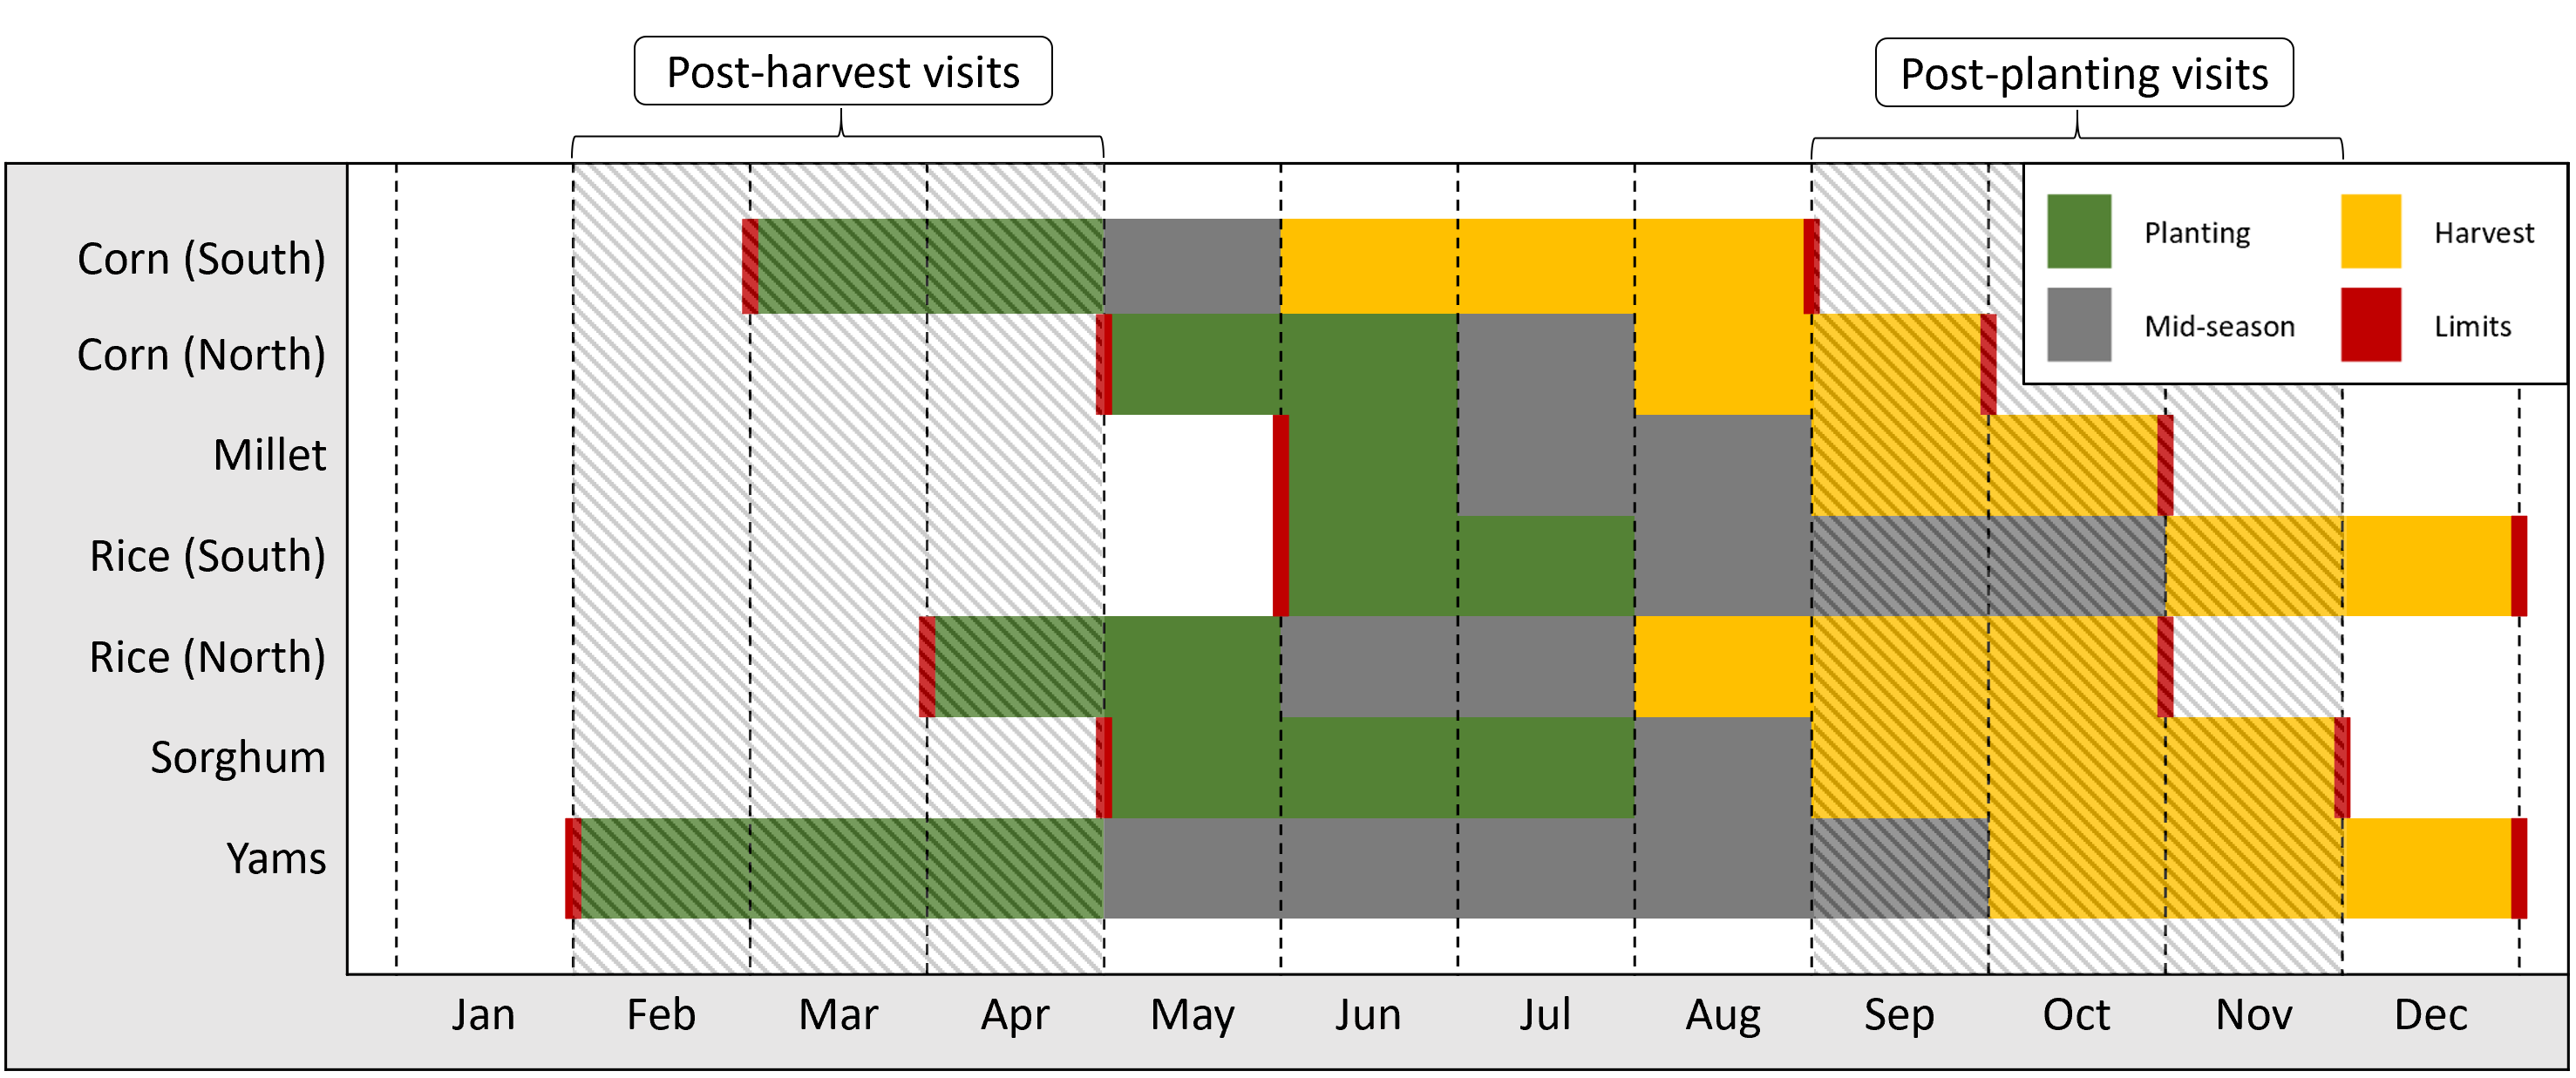
\includegraphics[scale=0.522]{../outputs/growing_season.PNG}
    \caption{Cropping seasons for selected crops of Nigeria.}
    \caption*{\footnotesize{\textit{Notes:} The cropping schedule published in \citet[][p. 62]{shiru2019} is overlaid with the surveying schedule of the General Household Survey. The time windows during which post-harvest and post-planting visits took place are indicated by the crosshatched areas.\\ \textit{Source:} \citet[][p. 62]{shiru2019} and \citet{NBS2020}.}}
    \label{fig:growingseason}
\end{figure}

In the following empirical exercise, the climate variables PRE, TMN, TMX, and TMP \footnote{DTR is omitted as it would cause multicollinearity related to TMN and TMX. WET essentially measures the same phenomenon as PRE. VAP and PET are omitted as they have no clear theoretical connection to child labour and may cause problems with multicollinearity as well. FRS is omitted because there are no recorded days below freezing.} are passed to the spline function in equation \ref{eq:bspline} for months $\tau$ in the bi-annual time intervals $t$ of the child labour outcome variable. Table \ref{tab:time_correspondence} shows the correspondence of these two temporal scales for all six GHS visits (three waves) used. In fact, what \citet{NBS2020} call ``post-harvest" visits usually take place during the planting season, whereas ``post-planting" visits fall within the harvest. 

\begin{table}[h]
    \singlespacing
    \centering
    \caption{Time correspondence of CRU-TS variables.}
    \begin{tabular}{|p{1.2cm}|p{1.2cm}|p{1.8cm}|p{3cm}|p{3cm}|}
    \hline
    \raggedright \textbf{wave} & \textbf{year} &\textbf{visit ($t$)} & \textbf{visit type}  & \textbf{months ($\tau$)}\\
    \hline
    1 & 2010 & 1 & post-planting & AUG - DEC\\
    1 & 2011 & 2 & post-harvest & MAR - JUL\\
    2 & 2012 & 3 & post-planting & AUG - DEC\\
    2 & 2013 & 4 & post-harvest & MAR - JUL\\
    3 & 2015 & 5 & post-planting & AUG - DEC\\
    3 & 2016 & 6 & post-harvest & MAR - JUL\\
    \hline
    \end{tabular}
    \caption*{\footnotesize{\textit{Notes:} Post-planting visits correspond to August thru December, whereas post-harvest visits are assumed to aggregate information from March thru July.\\ \textit{Source:} author's own compilation.}}
    \label{tab:time_correspondence}
\end{table}

Based on this correspondence between $t$ and $\tau$, I can now offer more specific insight into the variables that are included in the climate vector $\mathbf{c}_{it}$. Some of the climate variables are cumulative by nature and can, therefore, be aggregated by adding the monthly observations up over the five month periods associated with each visit. This concerns the variable PRE. Other variables - notably temperature - are mean values of daily observations.

Alas, the use of monthly average climate data attenuates much of the variation in daily weather and masks the importance of extreme temperatures to some extent. To not make matters worse, I do not average the monthly maximum and minimum temperature values further. Rather, the variables TMN and TMX are aggregated by choosing out of the five months associated to each visit the one that lies furthest from the mean temperature in either direction. TMP itself is, on the other hand, averaged over each visit's time window.

\subsection{Correcting for selection bias}
\label{sub:sample_selection}

Plotting the dependent variable - children's weekly working hours including household chores -  in figure \ref{fig:censored} shows a cluster at zero due to the fact that most children do in fact not work at all. In statistical terms, the data is censored at zero due to a selection process that selects children into two groups - those who work and those who do not.\footnote{This is also known as the ``extensive margin'' of labour supply.} As a result of this unobserved selection process, the effects estimated by standard FE may be biased (\textit{viz.} selection bias). Thus, the approach presented above needs to be adjusted.

\begin{figure}[h]
    \centering
    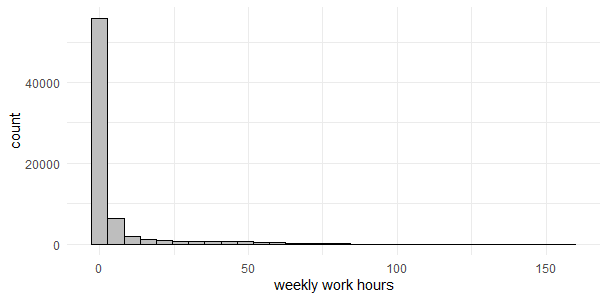
\includegraphics[scale=0.75]{../outputs/childworkchores.png}
    \caption{Child labour is censored at zero}
    \caption*{\footnotesize{\textit{Note:} Observed child labour hours including household chores, which were constructed from the GHS, are censored at zero. The graph was drawn from the pooled data of all six cross sections. The individual cross sections show the same pattern. \textit{Source:} Author's own compilation.}}
    \label{fig:censored}
\end{figure}

In cross-sectional applications, sample selection is commonly corrected for by modelling the selection process and the observed process in two separate equations. The Tobit estimator \citep{tobin1958,amemiya1984} and Heckman's selection correction \citep{heckman1979} method are the most used estimators of this kind. Unfortunately, these frameworks do not readily extend to panel data models with FE.\footnote{The issue is that the first equation, which models the selection process, is a binary choice model that is commonly non-linear. Unlike in linear models, which remain consistent when the fixed effect is treated as a parameter to be estimated, non-linear models are generally not consistent in this setting (This is the well known ``incidental parameters problem'').}

\citet{wooldridge1995}, however, proposes an alternative method for the estimation of panel data with unobserved, time-invariant effects and selection bias. \citet{semykina2010} extend this estimator to handle the presence of arbitrary correlation between unobserved heterogeneity and explanatory variables. While I shall briefly introduce this estimator, interested readers are referred to the original papers for a rigurous presentation of the material.

To be precise, the estimator proposed by \citet{wooldridge1995} is a correlated random effects model. It is, however, of the fixed effects (FE) variety ``in the sense that the unobserved component is allowed to be correlated with the observable explanatory variables, and we impose no distributional assumptions on the unobserved effect" (p.115). In addition, it does not require the idiosyncratic errors in the regression equation to have a known distribution, and they can have serial dependence of unspecified form.

Rewrite equation \ref{eq:linear_FE} as

\begin{equation}
    \label{eq:correlated_effects_model}
    y_{it}=x_{it}\theta + c_{i1}+u_{it1}, t=1,...,T,
\end{equation}
where, for ease of notation, $x_{it}$ is a $1\times K$ vector of explanatory variables that includes both the adapted climate variables $\bar{f}_{mit}$ and individual and household variables $\mathbf{x}_{it}$ from equation \ref{eq:linear_FE}. $c_{i}$ is the unobserved effect, and $u_{it1}$ is an idiosyncratic error.

Define a $1\times L>K$ vector of instruments, $z_{it}$, which is strictly exogenous on $c_{i1}$. Note that $z_{it}$ contains all elements of $x_{it}$ that are exogenous in equation \ref{eq:correlated_effects_model} and that $x_{it}$ and $z_{it}$ both contain an intercept.

Next, \citet{semykina2010} introduce selection by defining
\begin{equation}
    \label{eq:selection}
    s_{it}^*=z_{it} \delta_t + c_{i2}+u_{it2}, t=1,...,T.
\end{equation}
Here, $c_{i2}$ is an unobserved effect and $u_{it2}$ is an idiosyncratic error. Moreover, let
\begin{equation}
    \label{eq:selection_observed}
    s_{it}=1[s_{it}^*>0] = 1[z_{it} \delta_t + c_{i2}+u_{it2}>0],
\end{equation}
where $1[\cdot]$ is the indicator function. By definition, $s_{it}$ is a selection indicator that equals one if $y_{it}$ is observed, and zero otherwise. Note that in the current application, the data clearly shows that the censored variable  child labour $y_{it}\equiv \max(0,s_{it}^*)$ is observed for all $t$; we observe actual values for hours worked rather than a binary indicator only. \citeauthor{wooldridge1995} calls this ``partial observability of the selection variable" (\citeyear[][p. 120]{wooldridge1995}).

Assume that the model summarised in equations \ref{eq:correlated_effects_model}, \ref{eq:selection} and \ref{eq:selection_observed} holds. Moreover, let
\begin{equation}
    \label{eq:unobserved_effects_equation}
    c_{i1}=g(z_i)+a_{i1} = \bar{z}_i+a_{i1},
\end{equation}
where $g(\cdot)$ is an arbitrary known function. Equation \ref{eq:unobserved_effects_equation} is similar to the within transformation. It ``produces fixed-effects slope estimators when using a balanced panel''(\citeauthor{semykina2010}, \citeyear[][p. 377]{semykina2010}; see also \citeauthor{mundlak1978},\citeyear{mundlak1978}). In an unbalanced panel, however, it is different from the within-transformation because it models $c_{i1}$ as a function of $\bar{z}_i$, the elements of which are not distorted by selection. Therefore, ``the model is ideologically similar to fixed effects, but is free of selection bias''\citep[][p. 377]{semykina2010}. This makes it very attractive for the present case, since we are dealing with an unbalanced panel and sample selection.

For the case of an unbalanced panel, \citet{semykina2010} find that plugging Equation \ref{eq:unobserved_effects_equation} into Equation \ref{eq:correlated_effects_model} yields
\begin{equation}
    \label{eq:corrected}
    y_{it}=x_{it}\theta + \bar{z}_i \eta + \mathbb{E}(v_{it1}|z_i, s_{it}) + e_{it1},
\end{equation}
where, by construction, $\mathbb{E}(e_{it1}|z_i, s_{it})=0$ for $t=1,...,T$.\footnote{Note that it is not necessary that $\mathbb{E}(e_{it1}|z_i, s_i) = 0$. \citeauthor{semykina2010} emphasise that ``in fact, generally $e_{it1}$ will be correlated with selection indicators, $s_{ir}$, for $r \neq t$. This is a key benefit of the current approach: we can ignore selection in other time periods that might be correlated with $v_{it1}$''(\citeyear[][p. 380]{semykina2010}).} If $\mathbb{E}(v_{it1}|z_i, s_{it})$ were known, Equation \ref{eq:corrected} could be consistently estimated by pooled Two Stage Least Squares (2SLS). They also derive that, for $s_{it}=1$,
\begin{equation}
    \label{eq:WS10_main_equation}
    y_{it}=x_{it}\theta + \bar{z}_i \eta + \mu \hat{\lambda}_{it} + e_{it1},
\end{equation}
where $\hat{\lambda}_{it}$ is an estimate of the inverse mills ratio, obtained by probit. This, in turn, leads to the final procedure to estimate selection-corrected estimates from (unbalanced) panel data with unobserved, time-invariant effects.

\paragraph{Procedure 4.1.1. \citep[][]{semykina2010}:}
\begin{enumerate}
    \item For each $t$, estimate the selection equation by probit to get $T$ inverse mills ratios $\hat{\lambda}_{it}$.
    \item For $s_{it}=1$, use pooled 2SLS to estimate Equation \ref{eq:WS10_main_equation}. Use $z_{it1}$, $\bar{z}_i$ and $\hat{\lambda}_{it}$ as instruments.
    \item ``Panel-bootstrap'' the asymptotic variance. ``This involves resampling cross-sectional units (and all time periods for each unit sampled) and using the bootstrap sample to approximate the distribution of the parameter vector. The estimator is consistent for $N\rightarrow \infty$ and $T$ fixed''\citep[][p. 378]{semykina2010}.
\end{enumerate}
\hfill\qedsymbol\\
Applying this estimator to the use case specified in Equation \ref{eq:linear_FE}, I first run a Probit, regressing an indicator (1 if the child works, 0 otherwise) on the climate and household independent variables and retrieve the inverse mills ratios $\hat{\lambda}_{it}$. At the second stage, I estimate the equation
\begin{equation}
    y_{it}= \sum_{m=1}^M \beta_m \bar{f}_{mit} + \mathbf{x}_{it}\gamma + \bar{z}_i\eta + \mu \hat{\lambda}_{it} + \epsilon_{it}
\end{equation}
for all children who work non-zero hours by 2SLS. Household size is used as an identifying variable for selection.\footnote{\citet{semykina2010} call this an ``instrument''. The instrument should be strongly associated with the selection variable but unrelated to child labour hours. While household size is correlated more strongly with selection than with child labour hours, it remains a weak instrument, to be replaced whenever more suitable data is available.} Lastly, I bootstrap the asymptotic variance as suggested above. 200 bootstrap replications should be sufficient to obtain reliable standard errors \citep[][p. 47]{efron1994}.\footnote{I use the \texttt{XTHECKMAN} module \citep{rios-avila2021}, which implements the estimator of \citet{wooldridge1995} and \citet{semykina2010} in Stata.}

\section{Findings}
\label{sec:findings}

Table \ref{tab:results} summarises the output from four different regression models, all of which estimate the effects of climate variables on child labour hours. The first two columns show the coefficients on the climate variables from a pooled Ordinary Least Squares (OLS, Model (1)) and a panel regression with unit Fixed Effects (FE, Model (2)). The third column presents the coefficients obtained from the Correlated Random Effects (CRE, Model (3)) model proposed by \citet{wooldridge1995} and \citet{semykina2010}. Unlike models (1) and (2), model (3) is a two stage model that corrects for selection bias.

Note that models (1), (2), and (3) use the climate variables in their level (and precipitation squared) rather than cubic b-splines. To further investigate nonlinearities of climate effects, model (4) combines CRE with cubic b-splines as discussed in the preceding section. The functional flexibility of b-splines comes, however, at the cost of interpretability which is reduced to directional, qualitative statements. Therefore, the most interesting coefficients in table \ref{tab:results} are perhaps those of model (3).

\begin{landscape}
\begin{table}[htbp]
\begin{center}
    \caption{Climate effects on weekly child labour: regression results.}
    \label{tab:results}

\begin{tabular}{l*{9}{c}}
    \hline\hline
Model &\multicolumn{1}{c}{(1)}&\multicolumn{1}{c}{(2)}&\multicolumn{1}{c}{(3)}& &\multicolumn{1}{c}{}&\multicolumn{1}{c}{}&\multicolumn{1}{c}{(4)}&\multicolumn{1}{c}{}&\multicolumn{1}{c}{}\\
Estimator &\multicolumn{1}{c}{OLS}&\multicolumn{1}{c}{FE}&\multicolumn{1}{c}{CRE}&& & &\multicolumn{1}{c}{CRE}& &\\
\cline{2-4}    \cline{6-10}
    \textit{cubic b-spline section} &-&-&-& &\multicolumn{1}{c}{1}&\multicolumn{1}{c}{2}&\multicolumn{1}{c}{3}&\multicolumn{1}{c}{4}&\multicolumn{1}{c}{5} \\
    [1em]
    Variable\\
    \hline
    \texttt{Precipitation (100 mls)}
    & -0.673\sym{***} & -1.023\sym{***} & -4.035\sym{***}&
    & -17.644\sym{***} & -18.669\sym{***} & -15.521\sym{***} & -24.795\sym{***} & -24.219\sym{***}\\
    &     (0.20)      &     (0.22)      &     (0.44)     &
    &     (2.35      &     (1.74)      &     (2.15)     &     (1.85)       &     (2.97)     \\
    [1em]
    \texttt{Precipitation squared}
    &  0.023\sym{*}   &  0.051\sym{***} & 0.241\sym{***} & & & & & & \\
    &     (0.01)      &     (0.01)      &       (0.03)   & & & & & & \\
    [1em]
    \texttt{Mean temperature (°C)}
    &  2.315\sym{***} &  1.008\sym{**}  & 4.118\sym{***} &
    & -4.961\sym{***} &  0.943\sym{}    & 2.417\sym{*}   & 2.095\sym{}      & 3.384\sym{*}   \\
    &     (0.17)      &     (0.33)      &     (0.55)     &
    &     (1.16)      &     (1.03)      &     (1.05)     &     (1.22)       &     (1.38)     \\
    [1em]
    \texttt{Maximum temperature (°C)}
    &  -1.24\sym{***} & -0.947\sym{***} & -1.701\sym{***}&
    &   2.583\sym{}   & -3.890\sym{***} & -3.611\sym{*}  & -2.910\sym{*}    & -6.238\sym{***}\\
    &     (0.08)      &     (0.09)      &     (0.19)     &
    &     (1.79)      &     (1.10)      &     (1.60)     &     (1.23)       &     (1.59)     \\
    [1em]
    \texttt{Minimum temperature (°C)}
    & -0.712\sym{***} & -0.259\sym{}    & -1.510\sym{***} &
    & 6.079\sym{**}  & 10.585\sym{***} & -2.524\sym{}    & 1.556\sym{}     & 0.774\sym{}    \\
    &     (0.06)      &     (0.14)      &     (0.23)      &
    &     (1.92)      &     (1.34)      &     (1.68)      &     (1.23)      &     (1.56)     \\
    [1em]
    \hline
    Unit FE & no  & yes & yes & & & & yes & & \\
    Zone FE & yes & yes & no & & & & no  & & \\
    Time FE & yes & yes & yes & & & & yes  & & \\
    \hline
    \textit{N} & 55,735 & 55,735 & 55,735 & & & & 55,735 & \\
    \hline\hline
    \end{tabular}
\caption*{\footnotesize{Estimates of climate effects on weekly child labour hours from pooled OLS (1), Fixed Effects (2), Correlated Random Effects \citep{wooldridge1995} with level variables (3), and Correlated Random Effects with variables transformed through five-fold cubic b-splines to account for non-linearities (4). \\
\textit{Notes:} \sym{*} \(p<0.05\), \sym{**} \(p<0.01\), \sym{***} \(p<0.001\). Standard errors in brackets. Models (1) and (2) use standard errors that are clustered for the 18,735 individuals who reoccur in the panel. Models (3) and (4) use panel-bootstrapped standard errors calculated from 200 bootstrap replications, clustered the same way. All four models control for age, age squared, sex, MPI, log of household consumption, and sector (rural or urban). Models (3) and (4) use household size as an instrument for selection in the first stage. Precipitation squared is used in models (1), (2) and (3) to account for nonlinearities while using the level variables. Models (1), (2) and (3) can be interpreted the usual way, which is not true for model (4) due to the variables in b-splines. \textit{Source:} Author's own compilation.}}
\end{center}
\end{table}
\end{landscape}

All models seem to agree that, on average, an increase in precipitation is associated with a decrease in child labour. This effect is not linear though since the coefficient on Precipitation squared is positive and significant in models (1) thru (3). In fact, plotting the predicted child labour hours from model (3) against precipitation in figure \ref{fig:effects} shows that the negative effect is strongest a the lowest levels of precipitation and flattens for precipitation volumes of more than 400 ml. One interpretation of this fact is that households who already experienced a high load of precipitation need not send their children to water their crops. An additional increase in precipitation has less negative effects on child labour because the remaining tasks need to still be carried out. This may also imply that droughts affect the production function more negatively than normal and even high amounts of precipitation would. This negative shock to the production function would also decrease the demand for child labour in accordance with the theoretical perspective of section \ref{sec:model}.

As for temperature, it seems that an increase in the mean temperature is, by itself, conducive to child labour. According to model (3), a one degree increase in mean temperature is associated with an additional 4 hours spent at work, conditional on that the child is working - this is a considerable increase, given working children's average of $8.4$ hours weekly. The effect may not be as linear as this coefficient suggests, though. Child labour tends to decrease at temperatures in the low twenties and only picks up at temperatures of 27 degrees celsius or more - giving rise to the U-shape depicted in the upper panel of figure \ref{fig:effects}. These nonlinearities are not reliably evidenced by the b-splines of model (4), though, which means that the increasing right side of the U might also be the effect of other covariates.

As for the tails of the temperature distribution, it seems that both maximum and minimum temperatures are negatively associated with child labour hours. In fact, the coefficients for both maximum and minimum temperatures are consistently negative and highly significant with the exception of some spline sections in model (4). 

Controlling for selection bias, model (3) suggests that a one degree increase in maximum temperature is associated with a decrease of child labour by almost two hours. The b-splines of model (4) show that this negative effect only takes shape for higher levels of maximum temperature, whereas the effects of the first quintile is non-significant and, therefore, statistically not different from zero. Interestingly, plotting the predicted values of child labour against maximum temperature, an increasing line is obtained - see the lower left graph in the upper panel of figure \ref{fig:effects}. It is unclear why this is, but it is reasonable to think that the negative marginal effect of maximum temperature is being outweighed by, for instance, the positive effect of a mean-temperature increase. 

One additional degree of minimum temperature decreases child labour by 1.5 hours on average. Once again, model (4) points to important nonlinearities in these effects. It suggests, that at the lower two quintiles, minimum temperature is actually associated with an \textit{increase} in child labour. This leads to the inverted U-shape depicted in the lower right graph in the upper panel of figure \ref{fig:effects}. This is a reasonable result, considering that there are no freezing days in the data and that Nigeria, more generally, tends to suffer from drought rather than from freezing. Therefore, in our case study, lower minimum temperatures are unlikely to negatively affect plant growth, leaving the need for labour input unaffected at lower minimum temperature.

\begin{figure}[H]
    \centering
    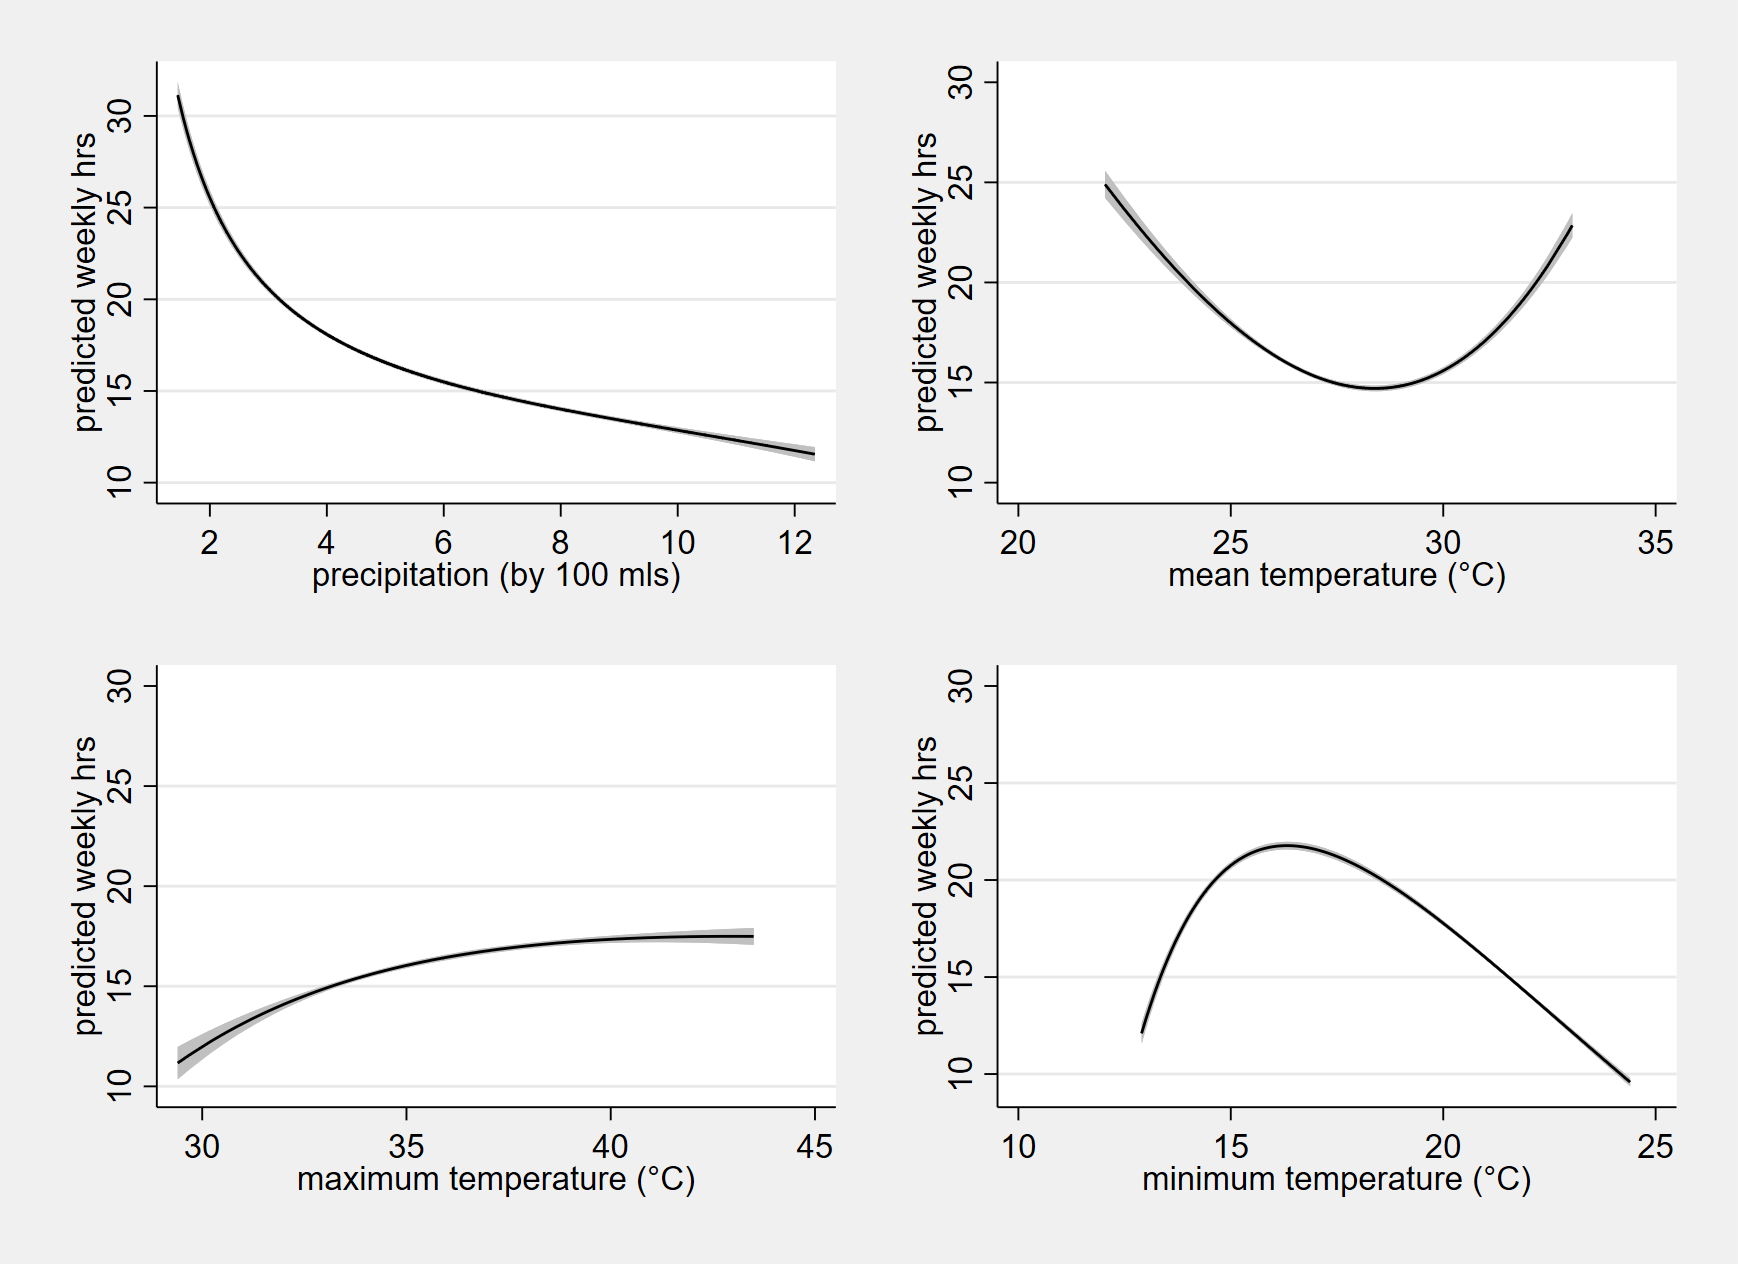
\includegraphics[scale=0.20]{../outputs/predicted_graph.png}
    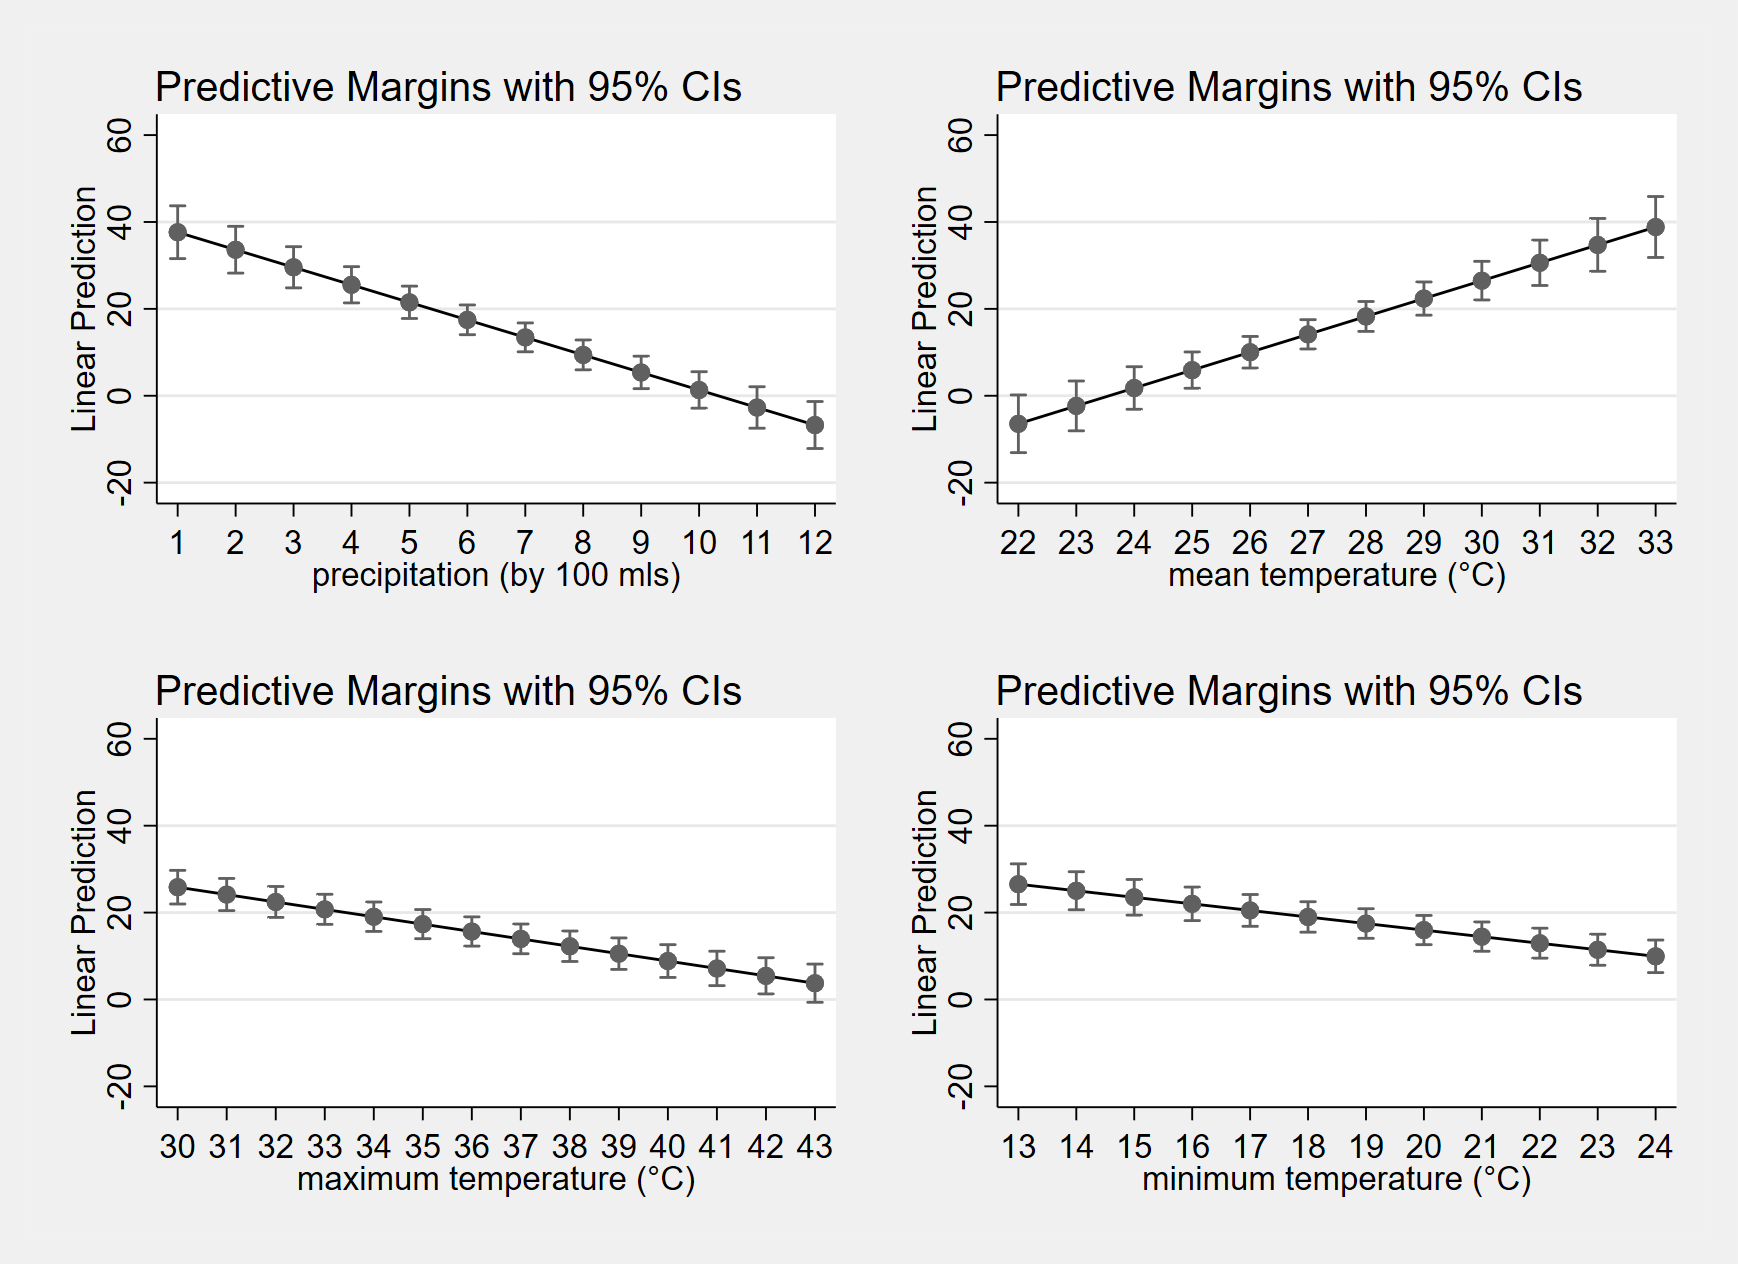
\includegraphics[scale=0.20]{../outputs/margins_graph.png}
    \caption{Predicted weekly child labour hours and marginal effects from Model (3).}
    \caption*{\footnotesize{\textit{Note:} The upper four panels of this figure graph a fractional polynomial fit on the predicted child labour from the CRE-level model (3) in table \ref{tab:results} against the climate variables precipitation (by 100 mls), mean-, maximum, and minimum temperature (by °C). 95 percent confidence intervals in grey. The lower four panels plot the marginal effects of the same climate variables, also with 95 percent confidence intervals. \\ \textit{Source:} Author's own compilation.}}
    \label{fig:effects}
\end{figure}

In summary, the analysis suggests that a permanent increase in mean temperature due to global warming leads to an increase in child labour. This effect may be somewhat counter-acted by the negative influence of weather variability on crops, which is also to be expected as the climate continues changing \citep{Pachauri2014}. Higher maximum temperatures seem to attenuate child labour supply in Nigeria slightly, which might be explained by a decrease in labour demand when there is less crop to harvest during hot periods. Minimum temperatures display mixed effects, forming an inverted-U shape with its turning point at approximately 16 degrees celsius. Before this point, it seems that child work increases with minimum temperature. Above it, the effect changes direction. Precipitation decreases child labour, in particular at very low quantities which points to the importance of droughts in the region. This last finding that child labour decreases in precipitation stands in contrast to earlier findings for Tanzania \citep{Dumas2020}, which evidenced a positive relationship.

Some of the control variables, which have been omitted from table \ref{tab:results}, also allow interesting insights. Somewhat surprisingly, the analysis finds no statistically significant effect of children's gender on the amount of their work hours. The effect of total household consumption spending is that with an aditional percentage point of household spending, children work 1.5 hours more. This is in line with the ``wealth paradox" that was first described by \citet{Bhalotra2003}; children of wealthier families tend to work more rather than less on average. Interestingly, though, the same is not true when employing MPI as an alternative poverty metric. The coefficient on MPI is non-significant.

\section{Conclusion}
\label{sec:conclusion}

This paper sought to describe the effects of climatic change on agricultural child labour. To this end, section \ref{sec:model} developed a simple household decision model rooted in the child labour literature. The main hypothesis of this model is that, all things equal, child labour should decrease with 'bad' weather and increase with 'good' weather, where bad weather affects plant growth negatively and good weather aids plant growth. The essential idea is that plant-growth is the one variable in the farm production function that is most closely linked to weather outcomes, which are in turn determined stochastically by the climate. As plants grow less, households' labour demand decreases and they react by decreasing the amount of child labour supplied, as they are assumed to be averse to child labour through the luxury axiom.

The hypothesis is tested in the empirical part of this study for the the case of Nigeria. The findings of this analysis are much more differentiated than the simple hypothesis posed. It is found that child labour tends to decrease, on average, with weather that is expected to hamper plant development. Extremely hot or cold temperatures and heavy rains are examples of this. However, the analysis also shows that child labour increases in mean temperature. This is counter-intuitive to the theoretical perspective of section \ref{sec:model}. The use of b-splines in one of the regression models, moreover, suggest the existence of important non-linear effects for all four climate variables.

Thus, the evidence points out the limitations of my simple theoretical model and, consequently, of its hypothesis. One major criticism that ought to be made is that it does not at all account for markets, including the credit and labour markets which both have proven to be influential factors in other studies \citep[e.g.,][]{Bhalotra2003,Dumas2013}. Their positive and negative effects (e.g., through selling labour or consumption smoothing) are not taken into consideration.

Moreover, there are some extensions that could have been made to the theoretical model's formulation of aggregate labour supply, of children's productivity in relation to that of adults, and the rather strict assumptions on time allocation. I chose not to make these extensions in the spirit of Occam's razor - instead, they are included in the annex. While these extensions might make the model's equations resemble real life a little better, they also would increase its complexity considerably. This would have been inefficient to do, given the limitations of the model in other domains. Rather than making the existing parts of the model more complex, future research should be geared towards integrating the roles of markets.  

Considering only the empirical section of this study, another criticism remains. I essentially employ what has been dubbed the ``dumb farmer approach" by \citet{Auffhammer2014}. My analysis does not take into consideration farmer's climate adaptation strategies, like changing farming practices or migrating. Therefore, the findings I present here are only really useful for the short term. They may, however, retain their validity for longer when focusing on the type of farmers implied by this study. It is, perhaps, reasonable to assume that poor subsistence-farming households would be ill-equipped to adapt to climate change, compared to more affluent ones. The effects of climate adaptation on child labour remain an important field of study, not least because one strategy to save labour costs when times get rough is to employ one's own children.

One more caveat concerns data availability. Due to the negative connotations surrounding the topic of child labour, parents may be inclined to under-report how much their children actually work. Therefore, the extent of child labour reflected in the data is likely lower than the real scope of the problem. Moreover, it is hard to come by high-definition climate data for the SSA region. While I use monthly climate data, it would be preferrable to have daily climate variables at one's disposal because monthly means already smoothen out a lot of variation from the data. The non-linearities reported here could be estimated more precisely with daily weather data. 

This study merely represents a first attempt at gauging the complex implications of the ongoing climate crisis for working children. It shows that climate effects on child labour seem to be non-linear and, in particular, that the projected increase in mean temperatures may stall ongoing global attempts at eliminating child labour by 2025 along with SDG 8. In a sense, this study also relates to the literature on measuring the `cost of carbon'. If child labour is considered a global bad, appropriate resources need to be used in order to counter it. Thus, this paper provides yet another reason for taking urgent action, in accordance with the Paris Climate Accord and the latest climate science, to limit global temperature rise in the 21st century to 1.5°C above pre-industrial levels.

\newpage
\small
%\nocite{*}
\addcontentsline{toc}{section}{References}
\bibliographystyle{apalike}
\bibliography{References}

\newpage
\appendix

\section{Annex: Extensions to the theoretical model}

The following pages present possible extensions to the theoretical model of section \ref{sec:model}. A comprehensive repository of information and files related to this project, including additional detail about the empirical analysis and its findings and an outline of the computational implementation, is available online at \href{https://github.com/mathiasweidinger/MPPTH}{www.github.com/mathiasweidinger/MPPTH}.

\subsection{Easing assumptions on time allocation}
\label{app:time_allocation}
The model in section \ref{sec:model} maintained the assumption that adults work all of their time, while children could set aside a share of their time $e\geq1$ to work effort. Alternatively, one could allow both children and adults to allocate their time between work and non-work. Keeping individual's time endowment standardised at 1, individual $i$'s work time share can be written as $l_i\in[0,1]$. The household's total aggregate time labour hours are obtained by summing $l_i$ across children: $\sum_{i=1}^{\hat{\imath}}l_i=L_C$. Conversely, all adult's labour input is captured by $\sum_{i={I-\hat{\imath}}}^I l_i=L_A$. In fact, this setup would allow for work time to vary not only between adults and children, but also across individuals of the same type.

\subsection{Children's productivity and adult supervision}
\label{app:adult_supervision}
In the model presented in section \ref{sec:model}, children were assigned an adult equivalence factor of $\gamma\in[0,1]$ that scaled their work units to those of adults, making child and adult work imperfect substitutes. \citet{Bar2009} extend this substitution axiom \citep{Basu1998}, contending that child labour must be supervised, using proportional amounts of adult labour, in order to be productive. In their model, children are employed when matched with an appropriate amount of adult supervision and left idle otherwise; child and adult labour are substitutes within a bound beyond which they become complements. Toddlers aside, this underlying assumption that unsupervised are completely unproductive might be too restrictive; Once instructed, even young children are able to replicate a multitude of simple tasks without constant monitoring. Rather than establishing child productivity, therefore, adult supervision can be thought to extend a low innate productive capacity. As a result, the household may make use of a given child's labour even when there is not sufficient adult time left to supervise it. This idea is developed further in this possible extension to the simple model.

To consider this formally, assume that child labour is necessarily less productive than adult labour by a factor $v(u)$, which specifies the adult-equivalence of child labour if a fraction $u\in (0,1)$ of adult labour is used to supervise the fraction $s\in (0,1)$ of child labour. Supervision generally increases children's productivity, such that
$$0< \underline{v}\leq v_0 = v(u=0)\leq v(0<u<1) \leq v(u=1)\leq\overline{v}\leq 1 \quad \forall u \in (0,1],$$
where $\underline{v}$ and $\overline{v}$ are the absolute boundaries of children's productive potential. I call $s$ the supervision rate, $u$ the intensity of supervision, $v(u)$ the technology of skill enhancement, and $v_0$ the adult-equivalence factor of unsupervised child labour (or ``raw skill"). In absence of supervision (viz., $s=0$), the initial adult-equivalent of aggregate child labour input is $v_0 L_C$ and the household's total labour input in this case is $L_{\mathcal{I}}=L_A + v_0 L_C$.

When supervision occurs, the technology of skill enhancement $v(u)$ exhibits monotonicity and decreasing returns to scale from supervision, meaning that

$$\frac{\partial v(u)}{\partial u}>0, \quad \text{and} \quad \frac{\partial^2 v(u)}{\partial u^2} < 0.$$
Moreover, it must hold that $v(u) > u \quad \forall u \in (0,1)$, since otherwise it would not be worthwhile to invest in supervision. Any monotonically increasing and concave function can be used to represent $v(u)$, provided it meets these few requirements. Panel (a) of figure \ref{fig:model} illustrates the shape of $v(u)$ by the example of the function $v(u)=v_0+(\overline{v}-v_0)u^{\frac{1}{3}}$, using four different values of $v_0$.\footnote{Note that $\overline{v}$ is unambiguously defined as follows from the definition of $v$ and $u$: $v(u=1)\leq\overline{v}\leq 1$ and $v(u)\geq u \quad \forall u \in (0,1) \iff v(u=1)=\overline{v}=1$.}

\begin{figure}[t!]
    \centering
    \caption{Supervision, child productivity, and labour supply.}
    \begin{subfigure}[t]{0.45\textwidth}
        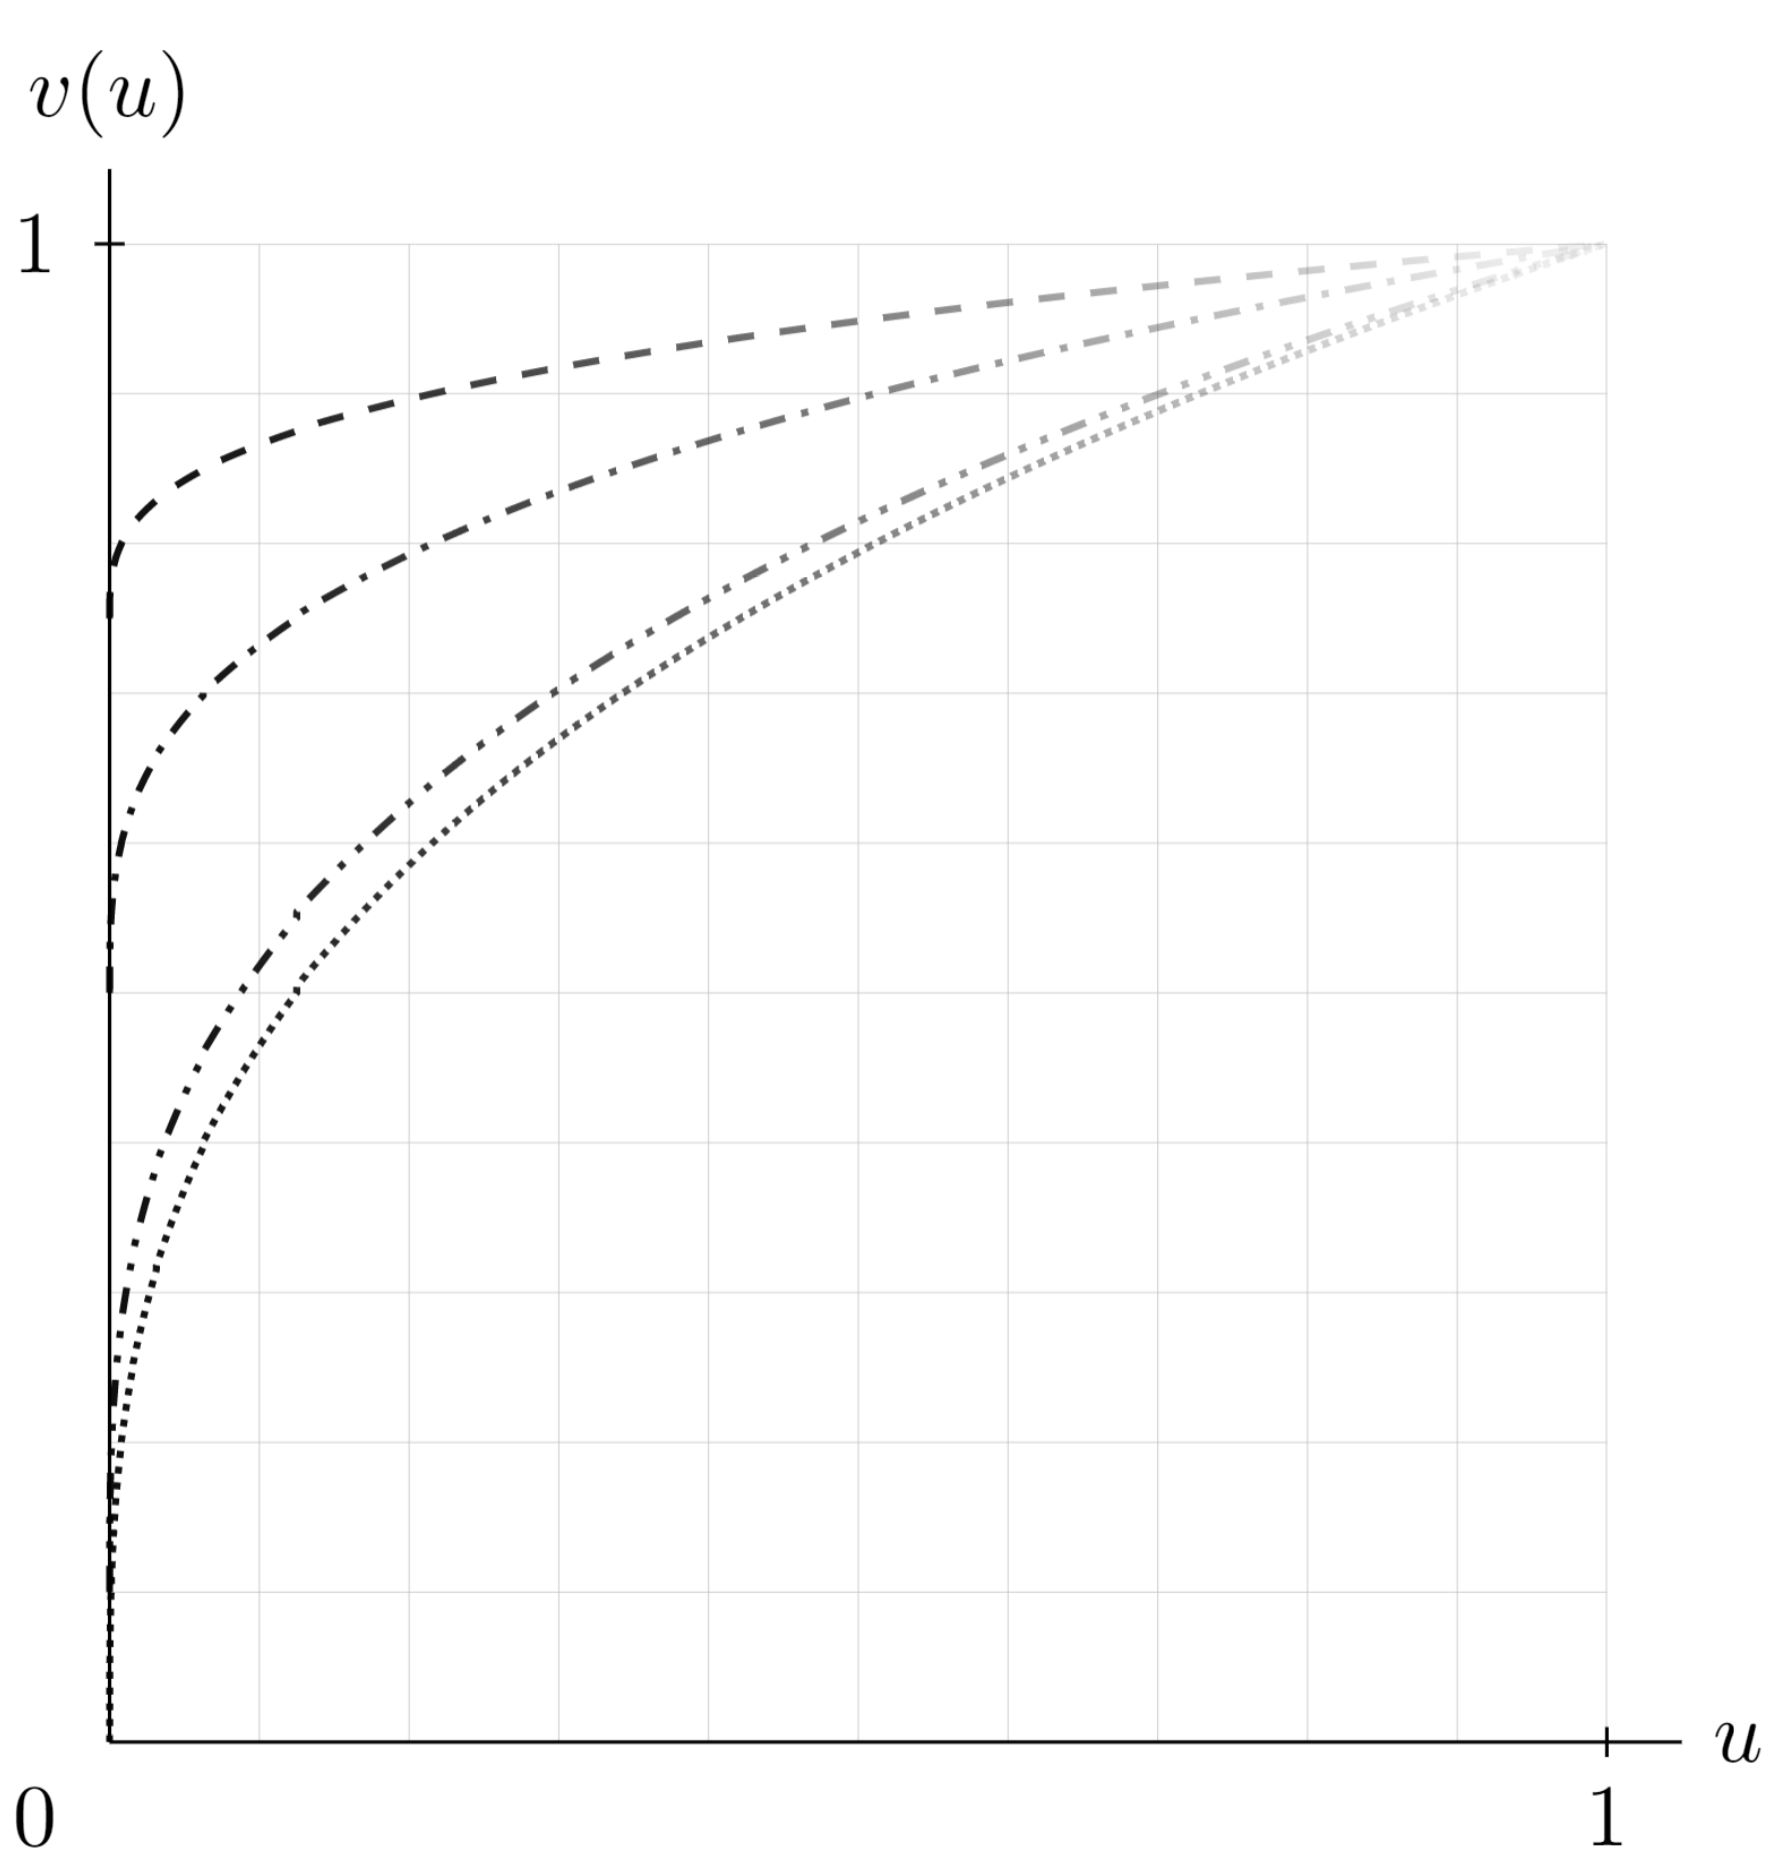
\includegraphics[width=\textwidth]{fig_skilltech}
        \caption{Technology of skill enhancement.}
    \end{subfigure}
    \hfill
    \begin{subfigure}[t]{0.45\textwidth}
        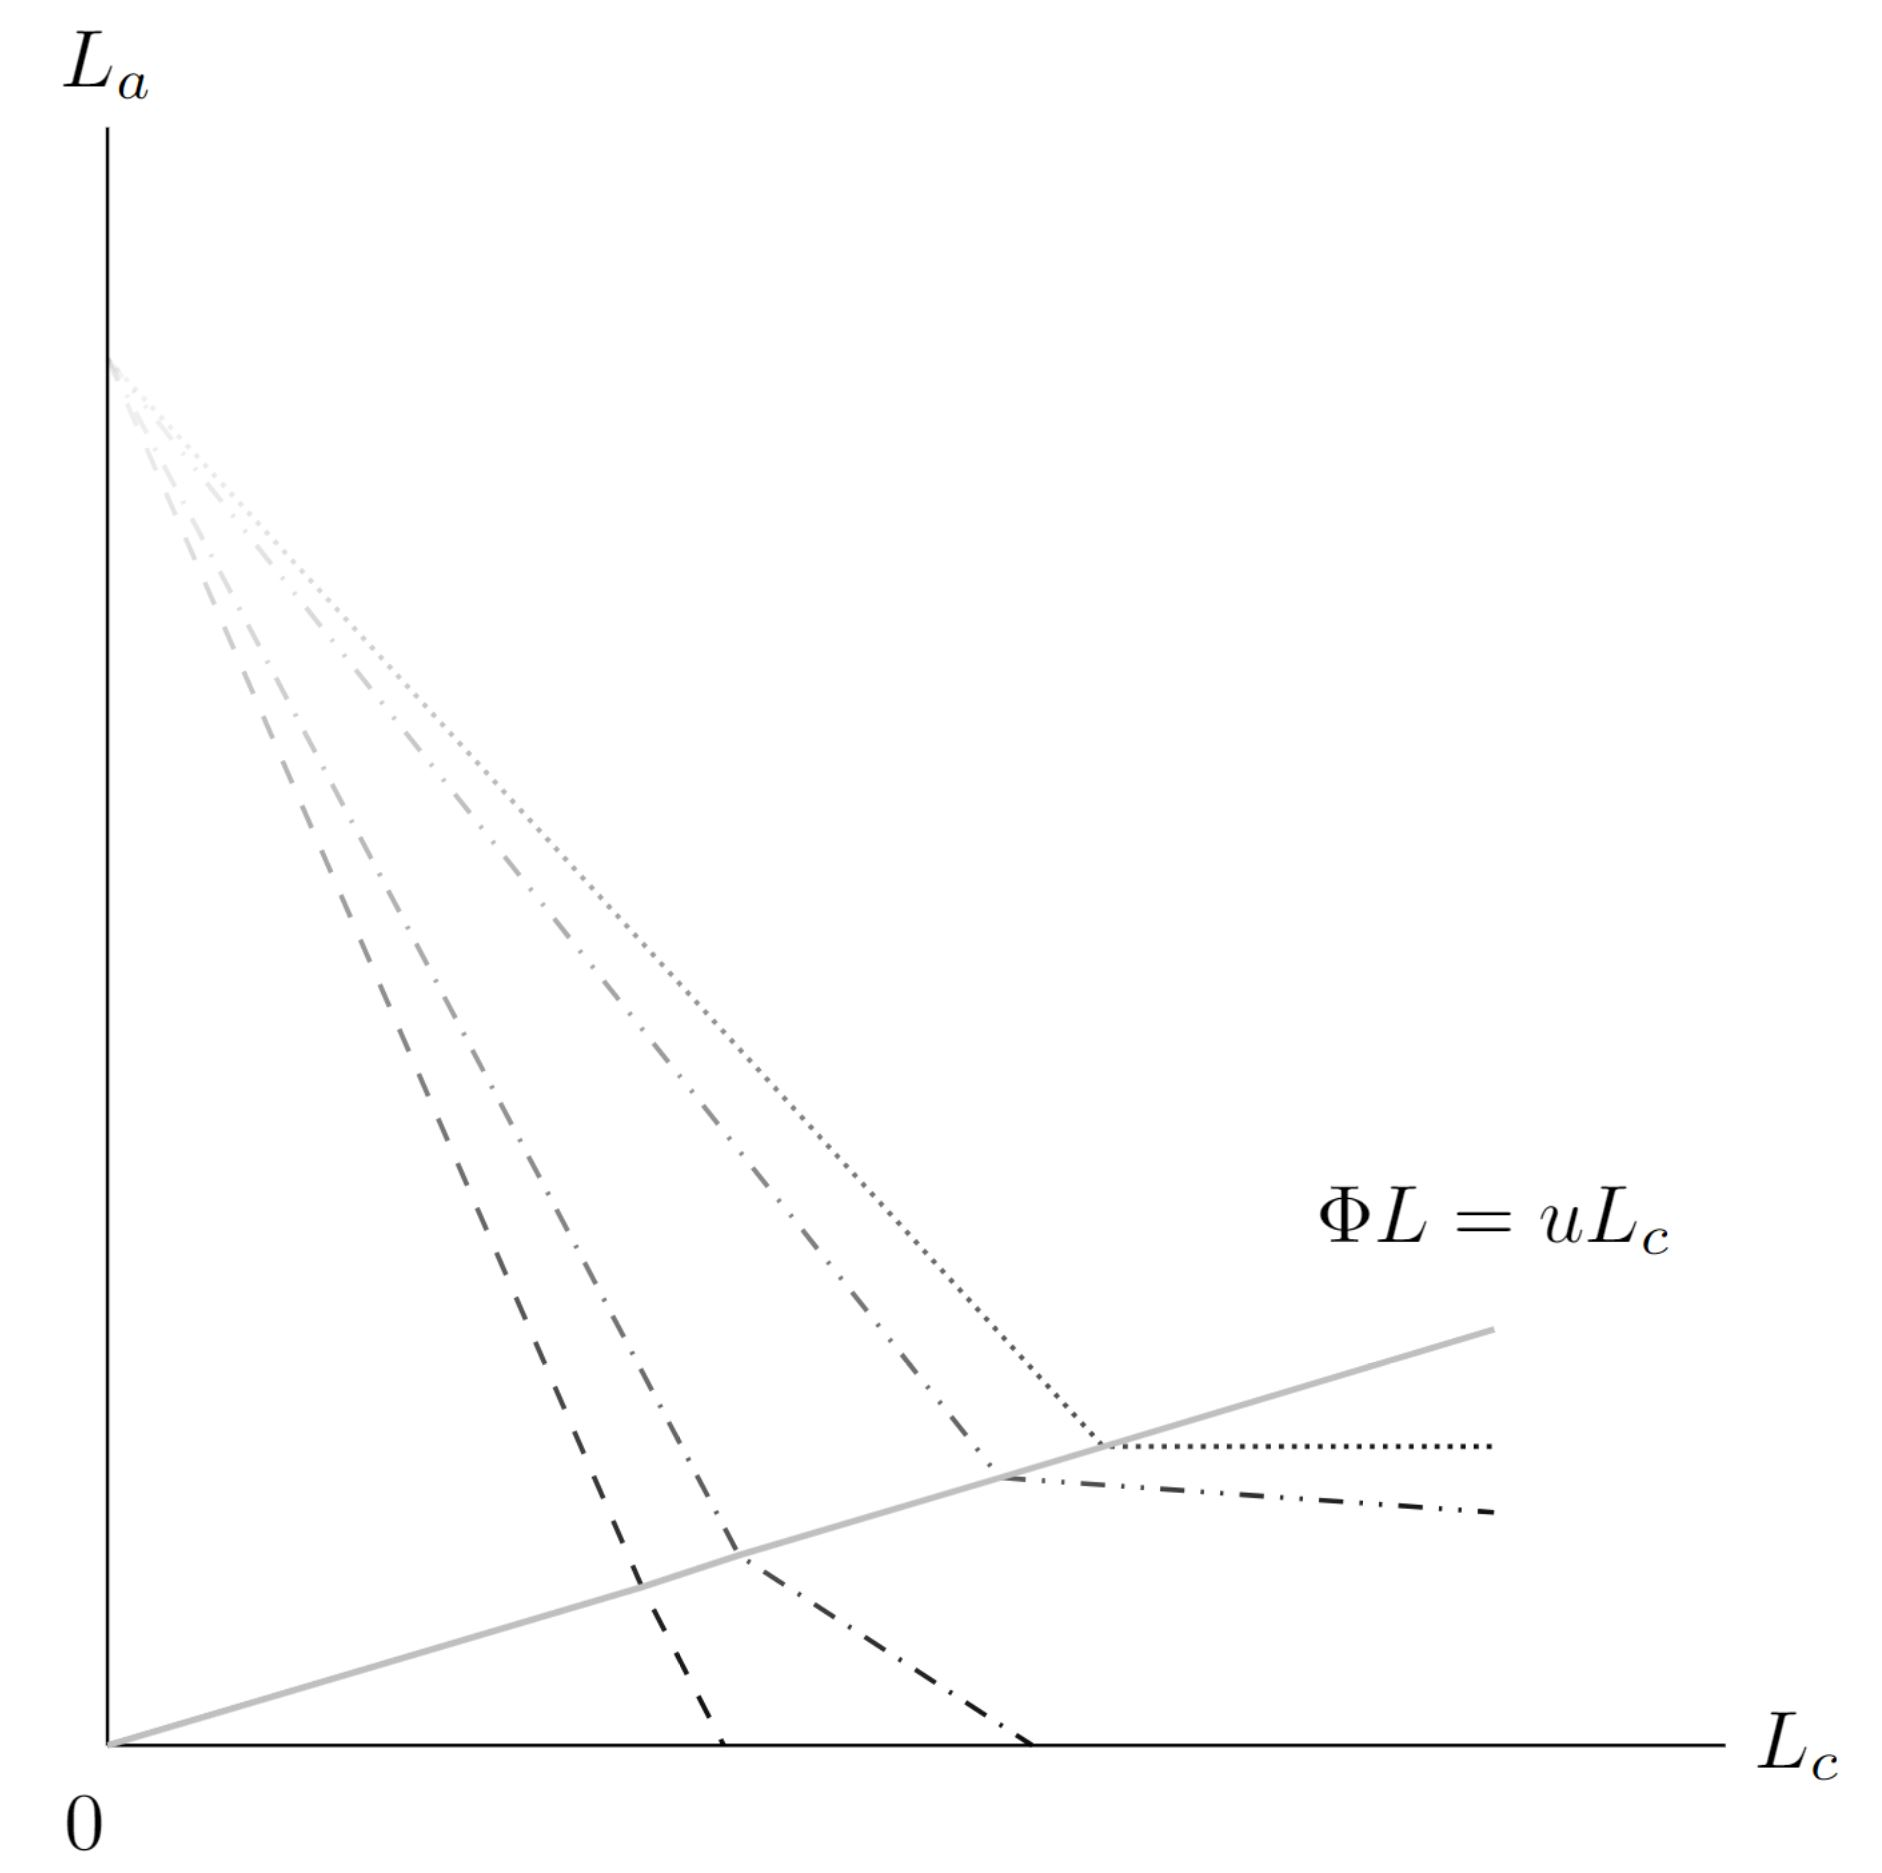
\includegraphics[width=\textwidth]{fig_isoquants}
        \caption{Effective labour isoquants.}
    \end{subfigure}
    \caption*{\footnotesize{\textit{Note:} (a) The figure graphs four versions of the function $v(u)=v_0+(\overline{v}-v_0)u^{\frac{1}{3}}$ for different values of raw skill $v_0$. The dotted curve corresponds to $v_0=0$ and the curves above it to $v_0=0.1$, to $v_0=0.5$, and to $v_0=0.75$ respectively. (b) The dotted isoquant corresponds to $v_0=0$, whereas the isoquants to its left correspond to $v_0=0.1$, to $v_0=0.5$, and to $v_0=0.75$ respectively. The upward sloping line in gray, which connects the isoquant kinks, is defined by its slope, the intensity of supervision $u$. \textit{Source:}  author's own compilations.}}
    \label{fig:model}
\end{figure}


The adult-labour equivalents of any given combinations of adult and child labour, considering the complementary of supervision in addition to the substitution between $L_a$ and $L_c$, can be captured by the household's effective labour supply:

\begin{equation}
\label{eq:labsup}
    L_{\mathcal{I}} =
        \begin{cases}
            L_A - s u L_C + s v(u) L_C + (1-s) v_0 L_C & \text{if} \quad s u L_C < L_A \\
            v(u) \frac{L_A}{u} + v_0 \left(L_c - \frac{L_A}{u}\right) \quad & \text {if} \quad s u L_C = L_A
        \end{cases}
        .
\end{equation}

This specification allows for the household decision maker to choose flexibly not only the levels of adult and child labour supply, but also the fraction of children to work with and without supervision, as well as the intensity of such supervision; all this in view of optimising the household's welfare. Setting $v_0=0$, $s=1$, $u<1$ and $v(u)=1 \quad \forall u$, equation \ref{eq:labsup} simplifies to the labour supply function in \citet{Bar2009}. Panel (b) of figure \ref{fig:model} plots combinations of child and adult labour, using the same values for $v_0$ as in Panel (a). The dotted curve on top corresponds to the Bar and Basu perspective that unsupervised child labour must be entirely unproductive (i.e. $v_0=0$).\footnote{For all functions graphed in figure \ref{fig:model}, it is assumed that $u=0.1$ and $s=1$.} Note that along each of the piece-wise linear functions in panel (b), the effective labour input $L$ stays the same, indicating that, holding other inputs constant, they are isoquants in the farm production.

\begin{align*}
    &\max_{c, e} (c-s)(1-e)\\
    \text{s.t.} \quad &(I-\hat{\imath})c+\hat{\imath}\beta c = f(L, \bar{K}, \theta)\\
\end{align*}
where
\begin{align*}
    &c \in \mathbb{R}^+ \text{ household consumption} \\
    &s \in \mathbb{R}^+ \text{ subsistence level of consumption} \\
    &e \in [0,1] \text{ child's time share in work} \\
    &I \in \mathbb{N}^{++} \text{ number of household members} \\
    &\hat{\imath} \leq I \in \mathbb{N}^{++} \text{ number of children in the household} \\
    &\beta \in [0,1] \text{ adult-equivalence factor of children's consumption} \\
    &L = (I-\hat{\imath})+ \gamma \hat{\imath}e \text{ Household's total labour supply} \\
    &\gamma \text{ adult-equivalence factor of children's work} \\
    &\bar{K} \text{ household's quasi-fixed capital stock} \\
    &\theta \text{ realisation of weather} \\
    &f(\cdot) \text{ agricultural production function, for which}\\
    &\frac{\partial f}{\partial L}>0, \quad \frac{\partial f}{\partial \theta}>0, \quad \frac{\partial^2 f}{\partial L^2}<0, \text{ and} \quad \frac{\partial^2 f}{\partial L \partial \theta}>0\\
\end{align*}
\end{document}